\documentclass[preprint,superscriptaddress,nofootinbib]{revtex4-1}
%~~~~~~~~~~~~~~~~~~~~~~~~~~~~~~~~~~~~~~~~~~~~~~~~~~~~~~~~~~~~~~~~~~~~~
\usepackage{amsmath}
\usepackage{amssymb}
\usepackage{amscd}
\usepackage{graphicx}
\usepackage{tabularx}
\usepackage{floatrow}
\usepackage{verbatim}
\usepackage{subfiles}
\usepackage{booktabs}
\usepackage{mathtools}
\usepackage{float}
\floatstyle{plaintop}
\restylefloat{table}
\usepackage{import}
%\usepackage[bottom]{footmisc}


%%Place New Commands Here

\newcommand{\cn}{\textbf{citation needed}} 
\newcommand{\eqn}{\begin{equation}}
\newcommand{\equ}{\end{equation}}
\newcommand{\fig}{\begin{figure}}
\newcommand{\fiu}{\end{figure}}
\newcommand{\tabitem}{~~\llap{\textbullet}~~}

 
\begin{document}
\title{Data Driven Modeling, Statistical Analysis, and Machine Learning for Additive Manufacturing}
\author{N.S. Johnson}
\author{R. Liu}
\author{X. Zhang}
\author{C.A. Brice}
\author{B. Kappes}
\affiliation{Department of Mechanical Engineering, Colorado School of Mines, Golden, CO 80401}

\author{H. Wang}
\affiliation{Department of Computer Science, Colorado School of Mines, Golden, CO 80401}

\author{B. Meredig}
\author{J. Ling}
\author{J. Saal}
\author{C.K.H. Borg}
\affiliation{Citrine Informatics, Redwood City, CA 94063}


\author{A.P. Stebner$^*$}
\affiliation{Department of Mechanical Engineering, Colorado School of Mines, Golden, CO 80401}


\begin{abstract}
In metal additive manufacturing (AM), materials and components are concurrently made in a single process as layers of metal are fabricated on top of each other in the (near) final topology required for the end-use product.
Consequently, a large number of processing degrees of freedom (tens to hundreds) must be simultaneously controlled and understood; hence, metal AM is a highly interdisciplinary technology that requires synchronized consideration of physics, chemistry, materials science, physical metallurgy, computer science, electrical engineering, and mechanical engineering.
The use of modern statistics-based approaches to modeling data sets with many degrees of freedom (known as machine learning) with metal AM can reduce the time and cost to elucidate and optimize the complex multidisciplinary phenomena.
Machine learning techniques have been used in materials science for several decades.
Most prolifically, the density functional theory community (DFT) rapidly adopted machine learning and has used it since the early 2000s for evaluating many combinations of elements and crystal structures to discover new materials.
This focused review examines the potential of machine learning in metal AM, highlighting the many parallels to previous efforts in materials science and manufacturing, and discusses new challenges specific to metal AM.
\end{abstract}

 
\maketitle

%\section{Motivation}

Metals-based additive manufacturing (AM) represents a potential paradigm shift in how products are manufactured, providing versatility in the type and design of parts produced by a single manufacturing facility, decentralizing manufacturing capability, and enabling novelty in the properties and design of the parts, to name but a few benefits AM offers. However, there have been significant roadblocks to fully realize AM's potential, particularly in the control of consistency and quality in part production and in the development of materials amenable to the AM process. Although decades of immense scientific and engineering work in industry, academia, and government have produced large advances in making AM a practical manufacturing solution, the metallurgical challenges facing AM persist. Computational materials simulation and the Integrated Computational Materials Engineering (ICME) approach have made strides in accelerating materials development, but the features that make AM such a departure from traditional manufacturing requires more uniquely suited problem-solving methods. In this paper, we argue that machine learning-based materials informatics is such a solution, capable of significantly accelerating the AM development process.


The 20th century saw the maturation of materials science and engineering as a field of study, enabling more rapid development of novel materials and materials manufacturing methods for specific applications. The process-structure-properties-performance paradigm transformed the combinatorial trial-and-error and intuition-driven materials discovery process into a problem of engineering a desired microstructure through designed processing. For instance, the history of turbine blade superalloy development is typified by advancements in control over microstructure through processing, including increasingly complex alloying recipes, multi-step heat treatments, and single-crystal casting. 

In the past decades, materials development has greatly accelerated to match the broader acceleration of general technology advancement. Computational materials science has enabled the prediction of microstructure from processing and of properties from microstructure, reducing the need for costly and time consuming experimentation. The Integrated Computational Materials Engineering (ICME) approach tightly integrates physics-based computational models into the industrial design process, allowing the desired performance requirements of a part to guide the design of a novel material. Examples include low-RE Ni superalloys for better turbine performance and lower cost and the Ferrium S53 alloy designed for corrosion-resistant landing gears. Both cases took materials development timelines from decades to years, demonstrating the practical capability of designing new materials within an industrial product timeframe. Generalizing this capability to more industries and further accelerating the process is the primary goal of the Materials Genome Initiative (MGI). 

Current AM capabilities are limited by materials-based problems which are uniquely difficult to solve with the above paradigm. The AM process itself is complex relative to traditional casting methods, including rapid solidification, vaporization and ingestion of volatile elements, and a complex thermal history, all of which vary with part location and require advanced computational tools to properly predict microstructure and properties. However, the lower cost and time barrier to entry for performing AM has enabled the rapid accumulation of experimental data, enabling the Edisonian approach for finding optimized AM processing methods and parameters of existing alloys. For AM, the ICME-based tools have been catching up, attempting to bootstrap legacy models to this data, with limited success. As such, current AM materials development is largely combinatorial, as the processing of legacy alloys are optimized with extensive design of experiments and AM-specific alloys with higher performance are just now being effectively developed.

It is within this context we argue that machine learning (ML) can accelerate the application of additive manufacturing. ML as a method for model development has shown wide application in the past years, in industries ranging from finance to social networking. The use of ML in materials has been relatively limited for a variety of reasons, primarily the lack of a curated and large dataset on which ML can operate. The MGI identified this as a primary problem for accelerating materials development, and there has been significant progress recently in infrastructure development for materials databases suitable for informatics tools such as ML. The difficulty in producing physics-based ICME models and the ability to rapidly and efficiently sample processing space in a combinatorial approach makes additive manufacturing an attractive use case for ML. Machine learning as a framework can couple the legacy ICME tools with the experimental data to produce much more accurate AM process-structure-property models and to automate the iteration of designed experiments for model improvement and optimized materials.

In this paper, we present our arguments for the use of ML to address AM challenges. We begin by detailing how ML could be applied to AM and the use cases we envision. Then we discuss existing AM models and how they could be integrated into a ML framework. Existing examples of ML as applied to materials and AM specifically are then reviewed. We conclude with a prospective outlook on the potential of ML for AM.

%I.	Motivation: Why would someone want to use ML approaches to solve AM problems?
%A.	The Edisonian Approach: Brute Force Search, Historical MatSci Approach: Trial and error requires luck and a lot of resources, takes a lot of time and money
%	Modern example of Edisonian approach: how long/cost to develop 304 welding wire or an Inconel? 
%B.	More Modern Advancements in Mat Sci Developments: Decades of effort have been made to reduce the time and cost to discover and deploy new materials/processes
%	Use specific development timeline examples
%		Combinatorial Example
%		ICME example Ð maybe Questek steel (Ferrium)? Or something recent? Using ICME and gains made there.
%C.	Machine Learning Provides Means to wrap all of these things together (combinatorial, ICME, traditional experimentation, etc. can be used in tandem):
%Automated Iteration with statistically measurable differences quantified
%	Great for AM b/c of high DOF space Ð feature identification challenging w/o statistics, etc.
%D.	Roadmap: Overview the flow of the rest of the paper.

%\section{Phrasing Additive Manufacturing as a Machine Learning Problem}\label{phrasing}

\subsection{The Assumptions Behind Machine Learning}
Ultimately, AM users desire a model that relates manufacturing parameters to AM material properties; i.e., a process-property model. In a functional form, this model can be written as
\eqn
f(x_1, x_2, ... , x_n) = \mathbf{y},
\label{fundamentalgoal}
\equ
where the inputs $x_i$ are $n$ different manufacturing parameters and the outputs $\mathbf{y}$ are measurable properties.

Currently, these process-property relationships are often developed by connecting separate process-structure and structure-property models of individual physical processes within AM.
For example, individual process-structure models are developed to relate : heat source parameters to melt pool topologies \cite{Khairallah2016} using the finite element method or similar computational techniques; melt pool topologies to solidification routes using thermal- and mass-diffusion models  \cite{Tan2011}; solidification to microstructure evolution using phase field methods \cite{Kundin2015}.
Separately, structure-property models are developed such as relating grain orientations and stress to material properties using crystal plasticity \cite{Pal2013, Pal2014}.
It is then by making connections between individual process-structure and structure-property models that researchers relate process parameters to material properties.
This understanding-through-sequential-modeling approach has the added detriment that the errors and uncertainty of each approach compound on one another, so that the final result is less accurate, more time consuming, and more expensive than the direct build-break approach to develop process-property relationships.
Machine learning is not a complete replacement for these traditional approaches, but rather a complementary modeling approach that can accelerate or even automate that process of building connections across many degrees of freedom that span the many different individual phenomenon within AM processes.
Two assumptions are necessary when using machine learning:
\begin{enumerate}
\item \textit{The Relational Hypothesis}: A correlative relationship exists between the data input to the model and the response of the system.
\item \textit{The Locality Hypothesis}: \deleted[id=CB]{Different} parts manufactured at similar points in the design space will have similar properties.
\end{enumerate}

The first hypothesis is required for finding regression and classification functions that are physically accurate.
\added[id=CB]{Not entirely sure what this means.
Maybe a more generic statement could work.
Hypothesis implies that if we expect to be able to optimize a pathway for a particular output there should exist some relationship between the inputs parameters, or subset of, and the output.}
The second hypothesis is used to compare data and datasets, as well as to search and optimize through regression and classification algorithms.

\subsection{Unsupervised Machine Learning}\label{unsupervised}

Unsupervised machine learning algorithms are used to identify similarities or draw conclusions from unlabeled data by relying on the locality hypothesis.
Consider an experiment that varies three different manufacturing inputs $x_1, x_2, x_3$ and measures a single material property $y$.
In matrix form, the data are expressed as:

\eqn
\begin{split} 
\mathbf{X} &= \begin{bmatrix}
	x_{1,1} & x_{2,1} & x_{3,1} \\
	x_{1,2} & x_{2,2} & x_{3,2} \\
	\vdots & \vdots & \vdots \\
	x_{1,m} & x_{2, m} & x_{3, m} \\
	\end{bmatrix} \\
\mathbf{Y} &= \begin{bmatrix}
	y_1 \\
	y_2 \\
	\vdots \\
	y_m \\
	\end{bmatrix} \\
\end{split}\label{initialmeasure}
\equ

where $x_{i,j}$ is the $j^{th}$ measurement of the $i^{th}$ manufacturing input.
A distance metric can be defined between data points in the design space.
For example, data can be collected at two points $\mathbf{a} = (x_{1}, x_{2}, x_{3})$ and $\mathbf{b} = (x_{1} + \delta, x_{2}, x_{3})$ and treat these quantities as vectors.
Computing the $\ell _2$ norm of $\mathbf{a}-\mathbf{b}$ yields

\eqn
|| \mathbf{a} - \mathbf{b}||_2 = \delta.
\equ

\added[id=CB]{Is it important to define L2-norm / compare to L1-norm.}



The value and magnitude of $\delta$ gives an inclination about how similar $\mathbf{a}$ and $\mathbf{b}$ are.
If $\delta$ is close to zero, then a researcher can say that they are similar, or even the same if $\delta$ is exactly zero.
As $\delta$ becomes larger a researcher can say $\mathbf{a}$ and $\mathbf{b}$ become more dissimilar.
The concept of `similar' manufacturing conditions may be easy to assess by an experimentalist when tuning only a few parameters at a time.
When taking into consideration tens or hundreds of design criteria, sometimes with correlated inputs, elucidating similar manufacturing conditions becomes difficult.
This vector distance approach is a simple, yet effective first glance at similarity in a design space and is generalizable to $n$ many design criteria.

Let us say that $\delta$ is small and that $\mathbf{a}$ and $\mathbf{b}$ are similar manufacturing conditions.
Now, consider a third point in the design space $\mathbf{c} = (x_{1} + \delta, x_2 + \delta, x_3)$ that has not yet been measured.
Since $\mathbf{c}$ was manufactured at similar conditions to $\mathbf{a}$, as measured by $||\mathbf{c} - \mathbf{a}||_2 = 2\delta$, then we may say that $\mathbf{a}$, $\mathbf{b}$, and $\mathbf{c}$ are all similar to each other. If the locality hypothesis is correct then manufacturing with conditions $\mathbf{a}$, $\mathbf{b}$ and $\mathbf{c}$ should yield similar measurements of $y$.

At some point, a researcher will have a set of initial manufacturing inputs $\mathbf{a}$, $\mathbf{b}$, $\mathbf{c}$, $\mathbf{d}$, etc., and associated property measurements that have been tested.
Churning through the remainder of all possible manufacturing conditions becomes expensive and tedious quickly.
Instead, researchers can use similarity metrics to determine whether or not a future test is worth running.
Comparing the manufacturing inputs through vector distance gives a rough idea of the possible outcome before spending time and resources on running a test.
If the intent is exploring design spaces then manufacturing at conditions \textit{furthest away} from previously observed points may be the answer.
If looking for local maxima of quality, an operator would want to manufacture at conditions \textit{nearest to} the conditions currently known to have high quality.

Using vector distances as metrics of similarities can produce results that are analogous to creating process maps \cite{Beuth2013}.
Process maps are used to divide $2$ dimensional plots of manufacturing inputs into regions of quality, or regions of different material responses.
The following demonstration is based on $k$-means clustering, a commonly used unsupervised machine learning clustering algorithm.

A researcher has acquired the datasets in Eqn. \ref{initialmeasure} and wants to partition $\mathbf{Y}$ into groupings of high quality parts and low quality parts.
However, there are several values of $y \in \mathbf{Y}$ that lie between two extremes and the cutoff for quality is not well defined.
It would be useful to use similarity metrics to find the best possible partition of quality.
To begin, the data set is partitioned randomly into two groups, $\mathbf{Y}_1$ and $\mathbf{Y}_2$.
The centroids $m_1$, $m_2$ (or centers of mass, in engineering) of each grouping can be calculated as

\eqn
	\begin{split}
		m_1 & = \frac{1}{|\mathbf{Y}_1|} \sum_{y_j \in \mathbf{Y}_1} y_j \\
		m_2 & = \frac{1}{|\mathbf{Y}_2|} \sum_{y_j \in \mathbf{Y}_2} y_j. \\
		\label{moment}
	\end{split}
\equ

where $|\mathbf{Y}|$ is the average value of a grouping.
The measurements were randomly partitioned at first; the goal is to re-partition each set so that similar measurements (similar levels of quality) are in the same set.
To do this, we can re-assign each set by

\eqn
	\begin{split}
		\mathbf{Y}_1 & = \{y_i : ||y_i - m_1||_2 \leq ||y_i - m_2||_2 \} \\
		\mathbf{Y}_2 & = \{y_j : ||y_j - m_2||_2 \leq ||y_j - m_1||_2 \}. \\
	\end{split}
	\label{reassign}
\equ

We can interpret the re-assignment in Eqn. \ref{reassign} physically: if a measurement initially assigned to set $\mathbf{Y}_1$ is closer in distance to $\mathbf{Y}_2$ then it is \textit{more similar} to the other set.
Thus, it is re-assigned.
Since the original partition was random it is likely that there are low quality parts mixed in with high quality parts - in other words, outliers exist in each partition.
Measuring the similarity of each data point to the mean of the groupings re-classifies these outliers into groupings that are more reflective of their quality.

Once re-assignment is complete the centroids in Eqn. \ref{moment} can be re-calculated and updated.
Then, data points are re-assigned once more based on how similar they are to the centroid of each partition.
If we have partitioned the input settings $(x_1, x_2, x_3)$ along with their corresponding measurements, then we have lists of input settings which are likely to give good/bad quality parts.
Further analysis can also be conducted, such as analyzing which regimes of inputs lead to good or bad quality - this is precisely what process maps represent.
The difference in this case is that $n$ many manufacturing conditions can be related to a quality metric simultaneously, with little to no human inspection or intervention.
Additionally, a researcher can dig further and analyze \textit{why} groups of input settings result in given quality for a material property.

\added[id=CB]{Should we show a clustering plot? Is it fair to say that we're just covering one unsupervised technique (clustering and dimensionality reduction). Do you want to cover clustering methods specifically (k-means, PCA, t-SNE)}
\added[id=CB]{It may also be useful to comment on how clustering differs from DoX}


\subsection{Supervised Machine Learning}
In a \textit{supervised machine learning algorithm} the goal is to find a relationship $T: \mathbf{X} \to \mathbf{Y}$ that best approximates the underlying physical relationship $f(\mathbf{x}) = \mathbf{y}$.
That is, supervised machine learning algorithms relate model inputs to labeled data.
It is not necessary to make any assumptions up front about the nature of $f(\mathbf{x}) = \mathbf{y}$ to find $T$.
We only need to rely on the relational hypothesis and assume the relationship exists.
The process of finding $T$ can take many forms, depending on the specific supervised ML algorithm being used.

One method to find $T$ is assume it is a vector that satisfies
\eqn
\mathbf{X}T = \mathbf{Y}.
\label{map}
\equ

A researcher usually seeks this relationship through the measurements they have observed; in this case, the measurements are stored in the matrices of Eqn. \ref{initialmeasure}.
A common method to find a vector representation of $T$, and a critical element in most machine learning algorithms, is through least squares regression. Least squares regression finds $T$ through a minimization problem, given by
\eqn
\min || \mathbf{X}T - \mathbf{Y} ||_{2}^{2}.
\label{leastsquares}
\equ
Equation \ref{leastsquares} can be interpreted analogously to similarity measurements for unsupervised algorithms: the closer that $\mathbf{X}T - \mathbf{Y}$ is to zero, the more similar $T$ is to $f(\mathbf{x})$. 

%\textbf{This next example was specifically requested by a co-author for an explanation of how LSQ is done. I think it detracts from the conversation.}\newline

%In many cases the relationship in Eqn. \ref{map} is going to be over-determined (or \textit{rank deficient}) because a researcher will have more measurements than input parameters. There will be more rows of Eqn. \ref{initialmeasure} than columns. This means that a unique solution does not necessarily exist. $\mathbf{QR}$ decomposition is commonly employed to solve the rank deficiency of Eqn. \ref{map}. $\mathbf{QR}$ decomposition involves finding a representation of $\mathbf{X}$ as the product of two matrices, $\mathbf{Q}$ and $\mathbf{R}$. The columns of $\mathbf{Q}$ represent the basis vectors of the design space that $\mathbf{X}$ inhabits. $\mathbf{R}$ is an upper-triangular matrix whose entries are the coordinates of the data points contained in $\mathbf{X}$. This representation of $\mathbf{X}$ has two advantages. First, it decomposes the manufacturing inputs contained in the rows of $\mathbf{X}$ into basis vectors with coordinates, an easily interpretable representation. Second, the nature of $\mathbf{QR}$ decomposition ensures that $\mathbf{R}$ is a square matrix. Thus, any equation involving $\mathbf{R}$ will have exactly as many variables as it has unknowns, removing the over-determinedness of the problem \cite{Poole2011}.

%Using the $\mathbf{QR}$ decomposition transforms the problem stated in Eqn. \ref{map} into
%\eqn
%\mathbf{QR}T = \mathbf{y}
%\label{QR}
%\equ
%Since $\mathbf{Q}$ is orthogonal, and therefore invertible, we can now solve the problem
%\eqn
%\mathbf{R}T = \mathbf{Q^{-1}} \mathbf{y}.
%\equ

The method of solving equation \ref{leastsquares} are many and varied; indeed, much of this review will focus on applying Eqn. \ref{leastsquares} to various problems through additive manufacturing.
The result is an approximation to the functional relationship $f(\mathbf{x}) = \mathbf{y}$.
A new point of interest in the design space $\mathbf{x'}$ can be chosen and its associated material property $\mathbf{y'}$ can be predicted by computing

\eqn
\mathbf{x'}T = \mathbf{y'}.
\equ

This simple example demonstrates how functional relationships can elucidate more information about design spaces.
Commonly used machine learning algorithms in materials science and engineering are given in Table \ref{ML}.
Note that the field of Machine Learning is evolving as fast as AM itself; hence Table \ref{ML} is by no means a comprehensive review of all machine learning algorithms, but rather is intended to provide a comparison between the form and function of some of the most widely adopted algorithms in materials science and engineering.



%~_~_~_~_~_~_~_~_~_~_~_~_~_~_~_~_~_~_~_~_~_~_~_~_~_~_~_~_~_~_~_~_~_~_~_~_~_~_~_~_~_~_~_~_~_~_~_~
\subsection{Tools of the Trade}
Based on the previous discussion and examples, researchers are equipped with two general tools to integrate into ICME approaches, namely: 

\begin{itemize}
	\item Measurement of similarity with distance metrics;
	\item Approximation of relationships $y=f(x)$.
\end{itemize}

These are the basic tools that will be used in the subsequent sections.
The method by which similarity is measured or $f(\cdot)$ is found is dependent upon the task at hand, the data being used, and the machine learning approach chosen.
In most cases, multiple appropriate approaches exist.

Throughout the rest of the article these two tools will be built upon and applied to a plethora of problems in AM.
In most cases, the discussion will be kept general - that is, the reader will be left to determine the best distance metric or regression tool to use.
In cases where specific methodologies already exist for a given problem the discussion will be more focused and exact.

\subsection{Design space considerations}
\label{subsec:DMC_design_space}
When attempting to optimize an AM workflow for a particular property, it is important to consider the size and complexity of the design space.
The size of this parameter space indicates the value of data-driven exploration.
While it may be most valuable to seed the design exploration by performing orthogonal experiments first(which could be determined using dimensionality reduction techniques), typical experimental conditions facilitate fine exploration of a small subset of the design space.
For example, a build plate of 44 samples is likely to be all of the same composition with each sample only differing by their part orientation on the build plate.
This hindrance suggests that seeding your design space from the currently available or past experiments will lead to desired output more quickly.

\begin{table*}
    \renewcommand{\arraystretch}{0.8}
    \setlength{\tabcolsep}{5pt}
    \begin{center}
        \begin{tabular}{@{}llll@{}}
            \toprule
            \hline
             Parameter & range & step size & levels \\ \midrule
            \hline
            \hline
            Skin/Contour/Core laser parameters: & & & \\
            Power & 100-200 W & 10 W & 10 \\
            Scan speed & 500-1000 mm/s & 100 mm/s & 5 \\
            Spot size & 50-100 $\mu$m & 10 $\mu$m & 5 \\
            Energy density & 1-5 J/mm$^2$ & 1 J/mm$^2$ & 5 \\
            \hline
            Build parameters: & & & \\
            Polar angle & 0-90$^\circ$ & 30$^\circ$  & 4 \\
            Azimuth angle & 0-180$^\circ$ & 90$^\circ$  & 3 \\
            Sieve count & 0-10 & 2 & 5 \\
            Amount of recycled powder & 0-100\% & 10\% & 10 \\
            \hline
            Other parameters: & & & \\
            Blade direction & 0-300 mm & 10 mm  & 30 \\
            Transverse direction & 0-300 mm & 10 mm  & 30 \\
            Hatch spacing & 0.1-0.50 mm & 0.1 nm  & 5 \\
            \hline
            \bottomrule
        \end{tabular}
        \caption{Typical AM design space set up for determining PSP relationships. Multiplying the factorial yields 10$^6$ possible experiments.}
        \label{table:design_space}
    \end{center}
\end{table*}

\subsection{Data pipeline}
\label{subsec:DMC_data}
There are a wide variety of computational tools associated with applying ML to materials science problems.
As there are not many large, robust, data sources for AM, developing a data pipeline should be a top priority for ML-focused AM teams.
Table\ref{table:data_tools} describes some common tools and how they may be useful to AM workflows.
It may be useful to breakdown the active learning process into four steps: identification, collection, condensation, and analysis.

\subsubsection{Identification}
Once an optimization goal has been set, it is useful to define the design space or number of experiments, that may be necessary to achieve such a goal.
A typical experimental design space may be dependent on two variables, the number of inputs and the level at which those inputs are varied.
For a typical build plate, it's possible to consider 10+ variables solely based on printing parameters.
Depending on the resolution to which each parameter should be varied, the design space will likely be too large to experimentally determine each value.
Table\ref{table:design_space}, illustrates potential parameters to consider for a typical AM design space.
While it is common to explore varying 2 to 3 of these parameters at a time, to fully explore this space would necessitate 10$^9$ experiments!

\subsubsection{Collection}
When optimizing a large design space, data collection may consist of two phases: uninformed collection and informed collection.
Initially, when no experiments have been performed, it is most useful to pick a subset of experiments that are most dissimilar to perform first.
In figure\ref{fig:SL}, due to the low dimensionality of the space, the most dissimilar experiments are easy to see.
For high-dimensionality design spaces, unsupervised learning techniques (t-SNE, PCA) may be useful to determine the most dissimilar experiments.

During both phases of data collection, it is useful to consider the number of format of initial data sources.
For AM, it is likely data will come from an instrument in the lab (i.e. XCT, mechanical testing) or previously recorded literature data.
When collecting data from literature tools like WebPlotDigitizer and Tabula are valuable for collecting data accurately and quickly.
Once data sources have been identified and some experiments have been performed it may be useful to unify disparate data into unique records.
For smaller projects, this could be as simple as transferring all relevant data to a csv.
For larger projects, users may want to consider an open data format, like JSON or SQL, to maintain robust data records.

\subsubsection{Condensation}
Condensing sparse data into an "ML-ready" dataset may vary greatly between projects but there are a few considerations specific to AM.
If multiple team members are collaborating on a project, it may be useful to consider standardizing input and output names ("Contour laser speed" vs. "Speed of contour laser").
This is important for both the research as it will ensure recorded properties are not incorrectly interpreted and for machine learning as unique strings are likely interpreted as different descriptors.
When working with large design spaces, Python packages like Numpy and Pandas do well to provide quick feedback for the density of a dataset and can highlight sparse areas of the design space.

During this phase, a resercher may also consider calculating features from raw data.
For example, the XCT may only record the size and position of pores but some pore statistics (min/max pore size) may prove useful for modeling.
During this step, the reseacher should apply their domain expertise to properly engineer useful features.

\subsubsection{Analysis}
Once some amount of a design space has been explored and the collected data has been condensed to the relevant properties of interest, machine learning algorithms may be able to guide which experiment to preform next.
Python packages like sklearn, tensorflow, keras, and OpenCV contain a variety of algorithms with well documented use cases.
For materials specific examples of implementing a sequential learning workflow, see the learn-citrination github respository.
Once an informative model has been generated, experiments should be optimized in batches that allow the model to improve over many cycles.
At this point, informed data collection, condensation, and analysis should be repeated until the design goal is realized.



\begin{table*}
    \renewcommand{\arraystretch}{0.8}
    \setlength{\tabcolsep}{5pt}
    \begin{center}
        \begin{tabular}{@{}llll@{}}
            \toprule
            Data source (instrument/software) & file type & processing tools & "ML-ready" output \\ \midrule
            \hline
            \hline
            X-Ray tomography (Zeiss Xradia Versa) & .tiff & image featurizer & vectorized image \\
            X-Ray tomography (TRACR) & .txt, .csv & Python (pypif, pandas, citriantion-client) & porosity statistics \\
            X-Ray diffraction (Panalytical empyrean) & .xy & Python (pypif, csv, pandas) & XRD features (\% desired phase) \\
            Optical microscopy (Keyence VHX-5000) & .tiff & image featurizer & vectorized image (grain size and distributions) \\
            Uniaxial tensile testing (MTS 370) & .xy & Python (Hough transform algorithm) & real-valued mechanical properties \\
            Composition (TOF-SIMS) & & Python (pymatgen, matminer, magpie) & composition feature vectors \\
            Semi-structured web page & .html & Python (requests, beautifulsoup) & csv-formatted records \\
            Semi-structured pdf (txt-based) & .pdf & tabula, AbbyyFineReader, Python (pdftotext) & csv-formatted records \\
            ML packages & & Python (sklearn, tensorflow, keras, OpenCV) & \\
            \hline
            \bottomrule
        \end{tabular}
        \caption{Common tools and packages for preparing data for ML applications}
        \label{table:data_tools}
    \end{center}
\end{table*}


\subsection{Preparing data for machine learning}

For materials synthesis applications, signal from machine learning models is often limited by the amount of data and the speed at which data can be collected.
Many standard algorithms are suitable to correlate high-dimensional inputs and outputs in the AM design space.

To prepare experimentally generated data for input to a machine learning model, python scripting and other automation tools are typically employed.
For AM synthesis optimization, data is generated at many disparate sources.
For example, after a build plate is printed, the porosity of each sample is determined through X-ray tomography while other mechanical properties are determined through tensile testing.
Data collected this way is typically resolved through a master record in which data from many instruments and synthesis steps is stored.
Also, storing these data in a human and machine-readable format allows for quick error checking and data maniuplation to be performed while still being accessible for machine learning.
Table XX highlights a variety of computational tools and Python packages and their relevance to AM synthesis optimization.


\begin{figure}
  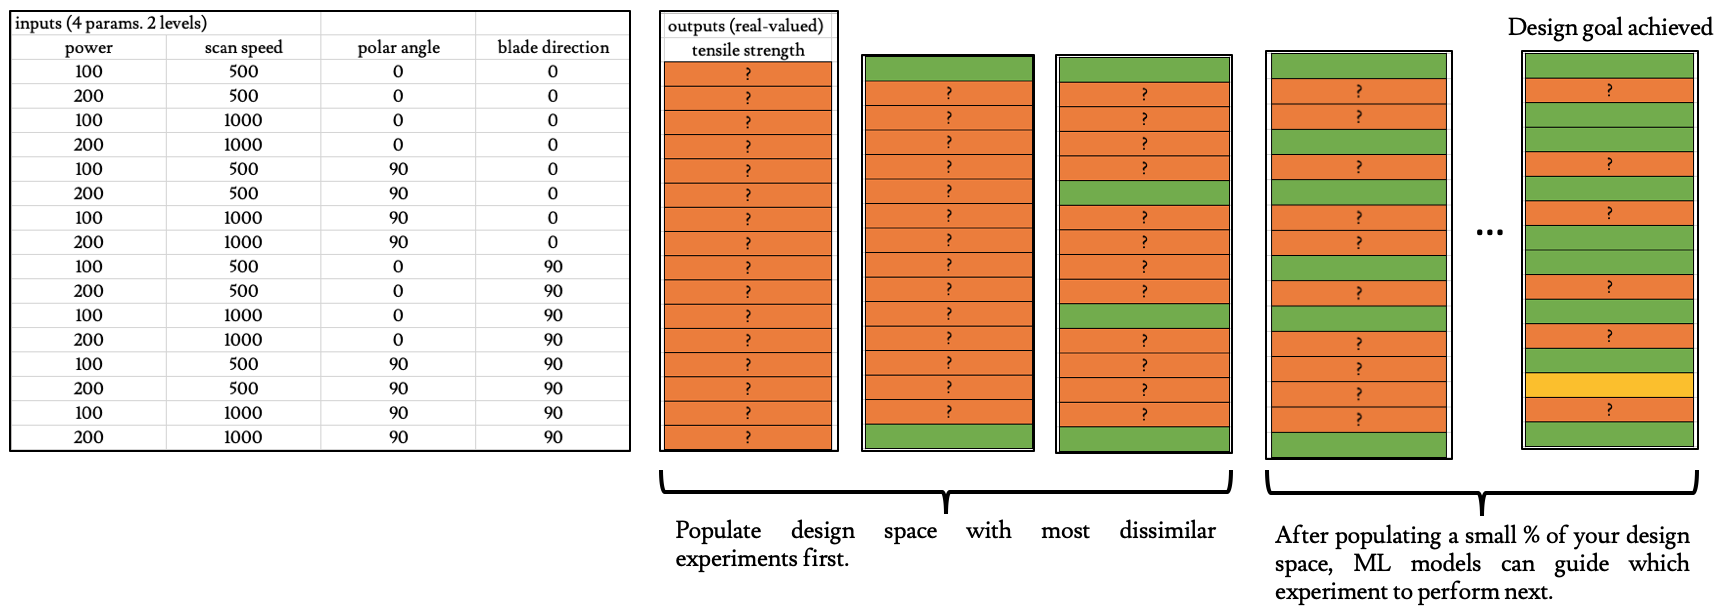
\includegraphics[width=0.9\linewidth]{SectionII/design_example.png}
  \caption{Illustrating a sequential learning workflow. In this example, there are 16 total possible experiments and
   4 experiments are performed for initial data collection. To reduce potential bias due subsampling of the input space,
  the most dissimilar experiments should be performed first. After populating some amount of the design space,
  machine learning should be used to begin informative data collection until design goal is realized.}
  \label{fig:SL}
\end{figure}

%%%
\begin{table*}[t]
\caption{Several of the most widely used machine learning algorithms that have been used in materials science are compared.} \label{ML}
\begin{tabular}{p{2.25cm}|p{2.25cm}|p{3cm}|p{4cm}|p{4cm}}
\raggedright Class of Algorithm & Examples & Applications & Strengths & Constraints \\ \hline \hline
Weighted neighborhood clustering & Decision trees, k-Nearest neighbor & \raggedright Regression, Classification, Clustering and similarity & These algorithms are robust against uncertainty in data sets and can provide intuitive relationships between inputs and outputs. See Ref. \cite{Quinlan1986} for a primer on clustering. & They can be susceptible to classification bias toward descriptors with more data entries than others. \\ \hline

\raggedright Nonlinear dimensionality reduction & \raggedright t-SNE, Kernel ridge regression, Multidimensional metric scaling &\raggedright  Dimensionality reduction, Clustering and similarity, Input/output visualization, Descriptor analysis, Regression, Predictive modeling &\raggedright These algorithms are robust against nonlinear input/output relationships and can provide intuitive projections of the material input/output space. For accessible examples, see Refs. \cite{Tenenbaum2000, Roweis2000}. & Projections can represent unphysical, difficult to interpret relationships. Global relationships can also be lost when nonlinear dimensionality reduction results are projected onto lower-dimensional spaces.\\ \hline

\raggedright Linear dimensionality reduction & \raggedright Principle component analysis (PCA), Support vector regression (SVR) & Dimensionality reduction, Clustering and similarity, Input/output visualization, Descriptor analysis, Regression, Predictive modeling & \raggedright This type of algorithm can produce orthogonal basis sets which reproduce the training data space. They can also provide quick and accurate regression analysis. For a primer on PCA specifically, see Ref. \cite{Bro2014}. & The relationships studied must be linear in nature, and these algorithms are susceptible to bias when descriptors are scaled differently. \\ \hline

Search algorithms & \raggedright Genetic algorithms, Evolutionary algorithms & Searching a material space to optimize on a certain condition, Lowest-energy state searches, Crystal structure prediction &  \raggedright Search algorithms are intuitive for material properties that can be described geometrically, such as topology optimization for weight reduction. They are efficient at searching spaces with multiple local extrema, such as finding local maxima of quality in multidimensional design spaces. &  These algorithms are highly dependent upon selection and mutation criteria. For a useful application of genetic algorithms to process characterization, see Ref. \cite{Grefenstette1986}. \\ 

\end{tabular}
\end{table*}
\added[id=CB]{move refs to their own column. A roadmap like this \href{https://scikit-learn.org/stable/tutorial/machine_learning_map/index.html} may be more informative than a table. It should be clear which methods are supervised/unsupervised}



%\input{SectionII/SectionII_cb.tex}
\paragraph{Current ICME Tools are Well Equipped to Integrate with an ML Framework}

The following section discusses how machine learning approaches can be used in current R\&D efforts in AM. This discussion includes how physics-based analyses, characterizations, and simulation methods may connect with different machine learning algorithms. Overall, the discussion is aimed at conveying how ML can be used to automate the generation of AM PSPP knowledge. Still, this article stops short of providing an exhaustive review of either machine learning algorithms or additive manufacturing. Instead, the intent is to introduce how ML approaches can be connected to AM research. The algorithms that are discussed were chosen because they were previously demonstrated in a materials science and engineering application \textbf{or} because the possible application of an algorithm to AM was clear and immediate. Similarly, the additive manufacturing problems addressed are not all-encompassing; they are merely a few that may be immediately addressable with machine learning approaches. 

%~%~%~%~%~%~%~%~%~%~%~%~%~%~%~%~%~%~%~%~%~%~%~%~%~%~%~%~%~%~%~%~%~%~%~%~%~%~%~%~%~
\subsection{Experimental Methods and Manufacturing Design}
\subsubsection{Alloy Design}
%\begin{figure}
%	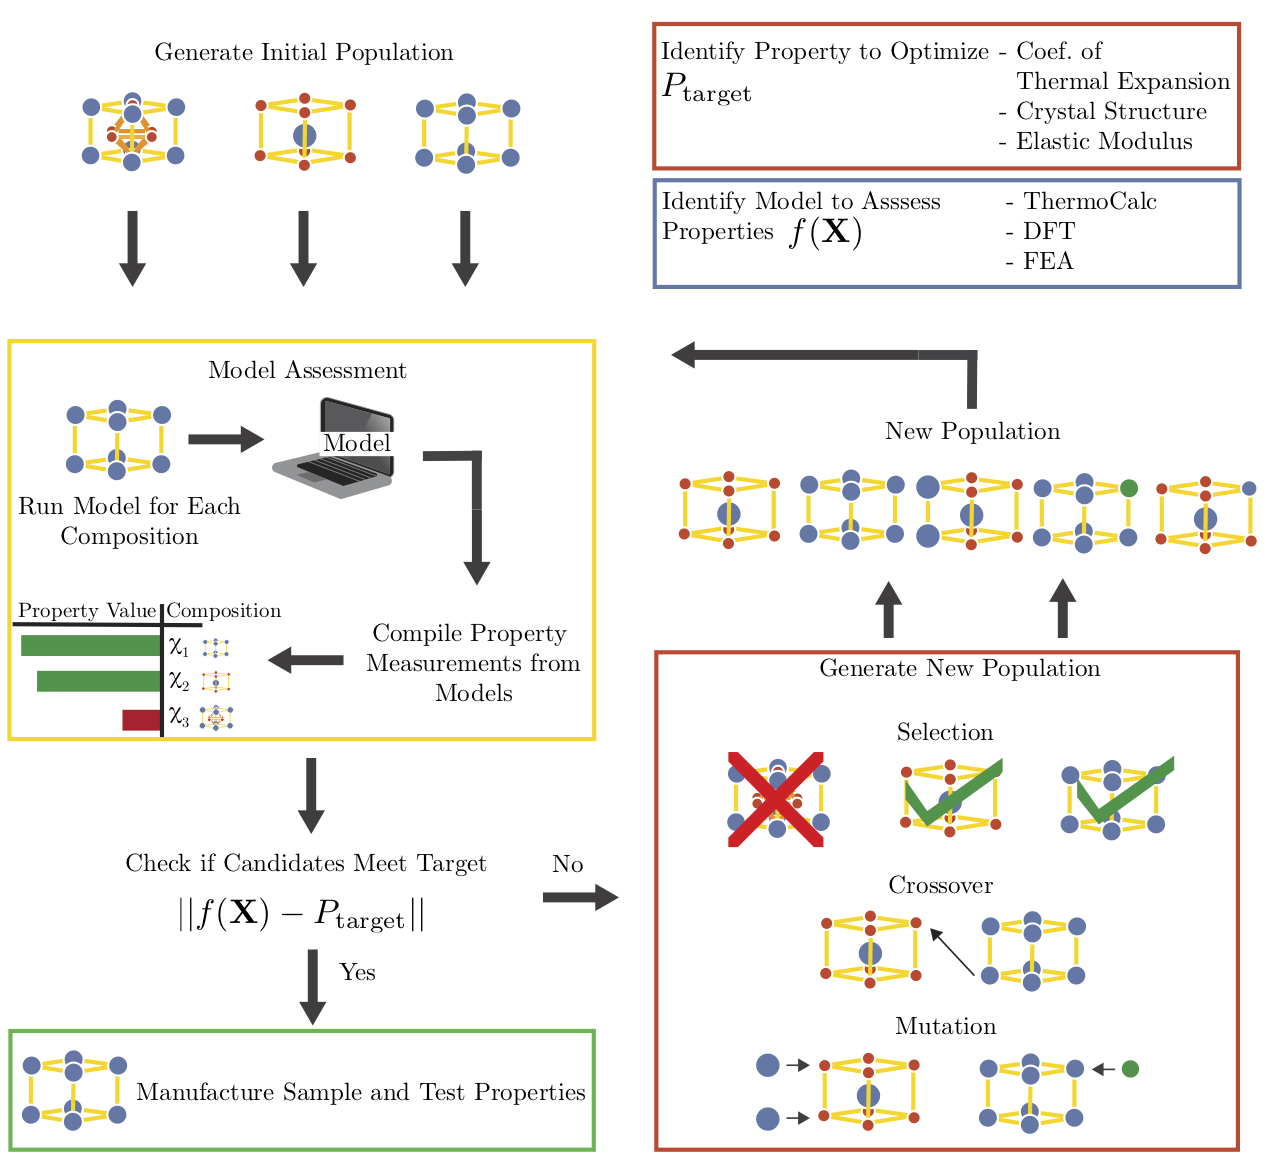
\includegraphics[width=1\linewidth]{Images/AlloyDesign}
%	\caption{}
%	\label{}
%\end{figure}
Choice of alloy impacts the physics of AM from start to finish, starting with the optics of energy sources incident on feedstock and ending with the material properties of the final part. For example, the reflected/absorbed intensity of lasers on powder beds is determined by the powder's composition \cite{Boley2016, Trapp2017}. The density of feedstock, both intra- and inter-granular density, plays a role in final part density \cite{Bi2013}. Conduction modes in the melt are partially determined by the thermal properties of the alloy \cite{Martin2017}. All of this is not to mention that different alloys exhibit different solidification kinetics, which can lead to drastically different microstructures after manufacture \cite{Collins2016}. 

Problems in the additive process can also be linked to composition such as vaporization of constituent elements due to rapid thermal fluxes, impacting the stoichiometry of melt pools and, ultimately, quality \cite{Brice2018}. Traditional engineering alloys sometimes need to be altered to improve compatibility with AM. Searching for new alloys specifically for AM may also be fruitful, as unique strengthening mechanisms can arise \cite{Brice2018, Wang2017}. Designing alloys for AM -- either altering currently used alloys or starting from scratch -- requires taking into consideration the compatibility of alloys' physical properties with AM. Alloy design for AM must take into consideration general alloy properties, like melting point, to feedstock-level properties, like vaporization temperature, to bulk alloy properties, like strength. Much of this information has been collated into databases that are compatible with design for AM. Alloy designers from AM should take advantage of these databases to search for new alloys for use in additive. 

Databases exist that contain alloy properties ranging from the reflectivity of the alloy to the mechanical properties of alloys in bulk. The International Crystal Structure Database (ICSD) contains crystallographic information for millions of compositions. The Linus Pauling files contains a range of material information, from atomic properties like radius and electron valency to crystallographic level information \cite{Villars1998}. In modern day, large databases such as AFLOWLib \cite{Curtarolo2012a}, the Materials Project \cite{Jain2013} and more allow users to search through large databases of relevant alloy information to find one that matches a desired property. Searching through large databases of information to find optimal compositions for manufacturing is actually one of the earliest materials informatics problems ever addressed. Methods exist to perform these searches in a fast, automated way. These methods are referred to as database mining, a data-driven materials design approach.

A study by Martin et al. used database mining to find micronucleants for Al alloys in powder bed manufacturing \cite{Martin2017}. Part of the design process is identifying which alloy properties are important for the desired application. Heterogeneous nucleation of Al grains was the desired outcome of Martin's study. To induce such nucleation, Martin et al. searched for possible nucleants whose crystallographic lattice parameters closely matched that of Al. This way, the Al grains would have a low-energy-barrier nucleating site from which to grow heterogeneously. Martin's study employed a search algorithm to search through 4,500 different possible nucleants and identify those with the closest-matching parameters. Ultimately, Zr was found to be the best candidate.

The same process employed by Martin -- identify the properties which need to be satisfied, then search for a material that is closest matching -- can be extended to many other alloy properties relevant to AM. Database mining was first introduced in material science to predict stable compositions, or estimate material properties from composition. Database mining has been successfully implemented to predict stable crystal structures \cite{Franceschetti1999, Fischer2006, Oganov2006} and predict material properties as a function of composition \cite{Ikeda1997, Gopakumar2018, Wu2018, Kirklin2013, Setyawan2011}. Some specially designed search algorithms have also been designed for improved speed in automated searches \cite{Wolf2000}. Successes have been found in designing Heusler compounds using high throughput search methods \cite{Roy2012}. Reviews of early high-throughput searches for compositions with ideal properties can be found in \cite{Gilmer1998, Koinuma2004}. The same search algorithms employed in these studies can be extended to the additive case.

A limiting factor in database mining is that designers are limited to properties which have been measured or calculated. We do not have information about the vast space of \textit{possible} materials. Consider a set of alloying elements for Ti such as $\{\text{Al}, \text{V}, \text{Zr}, \text{Cr}\}$. Researchers may need to test the impact of alloying composition on the dendrite arm spacing of Ti alloys. Phase field models exist which simulate the growth of and measure dendrite arm spacing as a function of a continuum of composition. A particularly efficient combined phase field/cellular automata model was implemented by Tan et al. precisely to model dendrite arm spacing in laser manufactured alloys \cite{Tan2011}. 

Modeling all possible combinations of $\{\text{Ti},\text{Al}, \text{V}, \text{Zr}, \text{Cr}\}$ is possible with coarse additions of alloying elements, but undesirable. Machine learning can aid in the process to find an optimal composition without modeling all possibilities. \textit{Genetic alogrithms} (GA) can search the space of possible alloys to find the optimal dendrite arm spacing. Genetic algorithms have been one of the most-used data driven approaches in materials science over the past few decades \cite{Morris1996, Ho1998, Wolf2000, Johannesson2002, Stucke2003, Hart2005, Oganov2006}.

The principle of genetic algorithms is to evaluate the \textit{fitness} of a population of candidate alloys against a \textit{fitness function}. The fitness function is a method of evaluating how well a candidate alloy meets a criteria.

As a thought experiment, consider using the CALculation of PHase Diagrams (CALPHAD) method as a fitness function. It can be run for candidate compositions -- in this case, various amounts of $\{\text{Al}, \text{V}, \text{Zr}, \text{Cr}\}$ alloyed into Ti -- and used to evaluate its compatibility with rapid solidification. This is similar to a study completed in \cite{Li2017}. Once a fitness function has been identified, the next step in a genetic algorithm is to represent candidate alloys as a \textit{gene}. 

We can represent a gene as \\

% You must have an empty line between text and the start of a table for some reason -- this is definitely going to be a problem later
\begin{table}[h!]
\begin{tabular}{cccccc}
	Alloy & $=$ & [$\chi_1$, & $\chi_2$, & $\ldots$, & $\chi_n$] \\
\end{tabular}
\end{table}
where $\chi_1$ is the species and weight percent of the first element (titanium, in this example), $\chi_2$ is the species and weight percent of the second element, up to $n$ elements. For example, Ti-6Al-4V would be represented as \\

\begin{table}[h!]
\begin{tabular}{ccc}
	 [0.9 Ti,  & 0.06 Al, & 0.04 V ] \\
\end{tabular}
\end{table}
The goal is to find the alloy with optimal dendrite arm spacing. First, a population of candidate genes needs to be generated, either randomly or by design. Two examples from a starting population may be \\

\begin{table}[h!]
\begin{center}
\begin{tabular}{ccccc}
	Alloy 1 & $=$ & [0.9 Ti, & 0.05 Al, & 0.05 V ] \\
	Alloy 2 & $=$ & [0.9 Ti, & 0.1 Zr] & \\
\end{tabular}
\end{center}
\end{table}
The thermodynamic properties of the various compositions, and therefore their compatibility with AM, is estimated by running a CALPHAD model for each composition. It is not guaranteed that the optimal composition is in this starting population.

Genetic algorithms select genes out of the current population -- called the parent generation --  to proceed to another generation of model assessment -- called the child generation. Selection consists of keeping the best performing compositions, say the top $10\%$, and discarding the rest. Genetic algorithms find optimal locations in the design space by relying on the similarity hypothesis. If one alloy is in the top $10\%$ of genes then it is possible that a similar alloy will also be high performing -- it may be even perform better. Once selection is done, the next step is to search the space near the best performing alloys from the parent generation.

Genetic algorithms generate similar compositions from those selected in the parent generation by making alterations to genes. One operation is \textit{mutation}, whereby entries of the genes are changed. For example, we could mutate alloy 1 by changing the composition:

\begin{table}[h!]
\begin{center}
\begin{tabular}{c|ccccc}
	\textbf{Parent Generation:} & Alloy 1 & $=$ & [0.9 Ti, & {\color{red}0.05} Al, & {\color{red}0.05} V ] \\ \hline
	\textbf{Child Generation:} & Alloy 1 & $=$ & [0.9 Ti, & {\color{green}0.02} Al, & {\color{green}0.08} V  ]  \\ 
\end{tabular}
\end{center}
\end{table}
\noindent where in the child generation the amount of V was increased, while the amount of Al was decreased. Another operation which may be performed is \textit{crossover} where entries of genes are added or interchanged. For example, one crossover operation may look like

\begin{table}[h!]
\begin{center}
\begin{tabular}{c|ccccc}
	\textbf{Parent Generation:} & Alloy 1 & $=$ & [0.9 Ti, & 0.05 Al, & 0.05 {\color{red} V} ]  \\
						 & Alloy 2 & $=$ & [0.9 Ti, & 0.1 {\color{green} Zr}] &              \\ \hline					 
	 \textbf{Child Generation:} & Alloy 1 & $=$ & [0.9 Ti, & 0.05 Al, & 0.05 {\color{green} Zr} ]  \\
						& Alloy 2 & $=$ & [0.9 Ti, & 0.1 {\color{red} V}] &              \\ 
\end{tabular}
\end{center}
\end{table}
\noindent where in the second generation V and Zr have been interchanged.

Selection, mutation, and crossover followed by model assessment and further selection, mutation, and crossover continues until the design criteria is met. The intuition behind genetic algorithms is that eventually the selection process is narrowed down to alloys within a given region of the design space such that further mutation and crossover do not produce new genes. Eventually, all the `fittest` genes as determined by the model will converge to be approximately the same composition. 

Genetic algorithms have been applied to alloy design for low and high temperature structural materials \cite{Ikeda1997, Kulkarni2004}, ultra high strength steels \cite{Xu2008}, specific electronic band gaps \cite{Dudiy2006}, minimum defect structures \cite{Anijdan2006}, exploring stable ternary or higher alloys alloys \cite{Hautier2010, Johannesson2002}, and more. For a review on the application of GA's to alloy design through the early 2000s see Ref. \cite{Chakraborti2004}.

Other machine learning algorithms have also been applied for classification and optimization of alloy compositions. Anijdan used a combined genetic algorithm--neural network method to find Al-Si compositions of minimum porosity \cite{Anijdan2006}. Liu et al. applied partial least squares to data mining of structure-property relationships across compositions \cite{Liu2006}. Decisions trees have been implemented for a number of different alloy optimization, such as predicting ferromagnetism \cite{Landrum2003} and the stability of Heusler compounds \cite{Oliynyk2016}. 
 
In the search for new alloys, some compositions definitely \textit{won't} be compatible with the additive process. It would be useful to identify these alloys up front or as quickly as possible. Additive can also be improved by machine learning algorithms which suggest the best materials or properties to test. A wide range of machine learning algorithms can be implemented to guide the entire experimental design process so that an optimized property is found as quickly as possible. 
\subsubsection{Design of Experiments}
Machine learning aids in investigations of AM by reducing the amount of experiments needed to characterize process-property relationships. Process-property relationships are typically studied through parametric analysis. Machine learning approaches like sequential learning model relationships in parametric studies to discover regions of the parameter space which will produce the most information about process-property relationships. 

Parametric analysis, broadly defined, is an experimental method of mapping independent variables, processing parameters usually, to their corresponding dependent parameters, material properties in this case. In additive manufacturing process parameters such as laser energy, speed, build direction, composition, layer height, and more are varied to study their impact on properties. Examples include relating build geometry to microstructure or surface roughness \cite{Antonysamy2013, Strano2013} or temperature history to microstructure \cite{Bontha2009, Nie2014}, or substrate temperature to residual stress development \cite{Chen2016, Brice2018}, or even entire manufacturing processes to microstructure \cite{Baufeld2011}. One of the most common types of parametric analysis is relating heat source parameters to all aspects of AM, such as part temperature history \cite{Bontha2006, Li2014}, microstructure \cite{Cherry2015, Jia2014}, mechanical properties \cite{Delgado2012, Khorasani2018}, residual stresses \cite{Wu2014, Denlinger2015}, and more.

Both engineering and scientific investigations of AM utilize parametric analysis. In the sciences, parametric analysis proceeds until a theory or model can be presented for a process-property relationship. In engineering, parametric analysis continues until an optimality criterion is met, such as maximum strength or minimum porosity. Both disciplines vary independent parameters and measure dependent responses; doing so provides information about the underlying phenomenon. 

\textit{Information} is any observation of process-property relationships. For example, observing that a set of laser parameters results in an equiaxed microstructure can be considered information because the researcher has gained an idea of the properties to expect from set processing conditions. Therefore, \textit{information gain} is any experiment which reveals a previously unobserved process-property relationship. Rigorous mathematical definitions of information and information gain have been defined, typically referencing back to Shannon's original formulation of information theory \cite{Shannon1948}.

Traditional design of experiments maximize information gain by dividing up parameter spaces to maximize distance between like experimental conditions. Machine learning driven design of experiments makes suggestions for future experiments based on the results of past experiments. It does not make any assumptions up front about correlations between design parameters. Rather, machine learning algorithms statistically model relationships between inputs and outputs and suggest the experiment which is statistically most likely to result in information gain. Design of experiments with machine learning algorithms can be adopted by augmenting traditional design of experiments with a statistical model.

The first step is to define the space of parameters which may impact properties, as is done in traditional design of experiments. The design space is all possible combinations of process parameters. As more parameters and finer step sizes are added, the size of the design space grows. Once the design space has been defined, the next step is to generate an initial dataset. The process-property relationships revealed in these initial tests will be the basis of an initial statistical model. 

After an initial dataset is generated, the researchers needs to define a \textit{response function} which interprets the relationship between parameters and material properties. One example is a regression model of the process parameters and material characteristics; this was the basis of a design of experiments study by Ling et al. \cite{Ling2017a}. In Ling's case, a random forest model was fit to design criteria from several different databases, such as a database of steel compositions, processing routes, and fatigue strength. The goal was to find the composition and processing route combination which had the highest fatigue strength in the dataset using as few experiments as possible. A benefit of random forest models is that they provide uncertainty estimates on predictions. This means that regions of the design space with high uncertainty can be identified.

Ling's machine learning-assisted design of experiments proceeded by suggesting experiments with a high uncertainty in their result as modeled by the random forest regression. The intuition is that predictions by the response function which have low uncertainty have enough data to characterize the process-property relationships in that region of the design space. Therefore, researchers can have high confidence in the material properties they will achieve if parts are printed at those conditions. Thus, the process-property relationship likely has enough information to pick an optimal condition or investigate further. Regions of the design space with high uncertainty do not have enough information therefore further experiments are required. Thus, machine learning algorithms suggest these regions of the design space for further experiments. When only varying a few parameters at a time, regions of the design space which need characterization can be easily identified. When varying tens of parameters in additive manufacturing these regions of the design space are not apparent. Furthermore, correlated inputs can be masked by the complexity of the process-property relationship. Statistical models can spot these correlated regions of the design space.

A regression model, such as that used by Ling, is only one way of assessing process-property relationships. A review article detailing many optimization algorithms for design of experiments can be found in Shan et al. \cite{Shan2010}. Adoption of machine-learning assisted design of experiments algorithms can rapidly increase the rate at which the relationship between AM process parameters and material properties are understood. 

\subsubsection{Topology Optimization} \label{sec:topology optimization}
Alloy design and experimental design focus around combinatorial screening of inputs to either search for \textit{new} properties or optimize on current properties. These optimizations reduce manufacturing cost, monetary or otherwise, and maximize performance capability. The same optimization can be applied to mechanical properties of parts. For structural materials, the goal is to optimize load bearing capacity or lifetime while minimizing the amount of material used. For aerospace, the goal is to minimize weight. Unique manufacturing geometries was one of the first intended applications of AM. Topology optimization (TO) focuses around exactly this task -- finding optimized topological structures for a given mechanical application. 

A filter is a mathematical operation which reveals information about a region of pixels/voxels in a mesh. Filters are most often represented as a product of a filter matrix with a matrix of mesh pixel values. Topology optimization proceeds by generating a CAD model of an AM part and modeling its performance, such as testing performance under mechanical load through an FEA simulation. Filters are applied to the CAD mesh which selectively removes material from the part. Then, the mechanical performance of the new part is modeled, followed by further material removal. This process proceeds until either a minimum weight/volume condition is met or the mechanical performance of the part is degraded.

In additive, topology optimization serves an additional purpose: TO algorithms can find un-printable regions of a part. Unsupported structures, low angle slopes, and certain part orientations during building are prohibited in AM because they will cause part deformation. An unsupported slope at acute angles can lead to part deformation and warpage \cite{Gaynor2016}. Sacrificial support structures also need to be considered during topological optimization, along with the number of free-hanging features and the orientation of the part during manufacture. Langelaar et al. developed an AM-specific TO algorithm which searches for regions of parts that have too little support for manufacture \cite{Langelaar2016, Langelaar2017}. Other additive specific algorithms have been designed for optimizing density of parts \cite{Zegard2016}. These algorithms augment the AM process, both by taking advantage of the ability to optimize unique geometries, and also by identifying regions of parts which are incompatible with AM.


%~%~%~%~%~%~%~%~%~%~%~%~%~%~%~%~%~%~%~%~%~%~%~%~%~%~%~%~%~%~%~%~%~%~%~%~%~%~%~%~%~

\subsection{Machine Learning Assisted Modeling of Additive Manufacturing}
As previously discussed, the design space of AM experiments is often vast (e.g., Fig. \ref{AMgene}). While the design of process parameters is often integral to the material design methods reviewed in the previous sections, there are some additional process-centric engineering objectives where machine learning methods may also be beneficial. This section reviews the use of machine learning algorithms to aid in computational design of additive manufacturing process developments. Martukanitz et al. published a full ICME investigation of AM \cite{Martukanitz2014}. There are two modeling scenarios that plague the advancement of AM: the case where a model exists but current numerical methods are too expensive to simulate the model; or the case where a model does not exist. Put slightly differently, in either case $\mathbf{y} = f(\mathbf{x})$ exists but cannot be computed in a reasonable amount of time; or $\mathbf{y} = f(\mathbf{x})$ does not exist. 

Machine learning algorithms have addressed both these cases. In the first case, ML algorithms provide an alternative numerical method for calculating $\mathbf{y} = f(\mathbf{x})$ based on experimental measurements of $\mathbf{y}$ and $\mathbf{x}$, or based on the results of previously run simulations. Machine learning algorithms have also been developed to help visualize trends in high dimensional spaces, allowing researchers to study complex relationships and ask deeper questions. For the second case, ML algorithms provide a form of $\mathbf{y} = f(\mathbf{x})$ from observations (measurements) of the relationship between $\mathbf{y}$ and $\mathbf{x}$.

\subsubsection{Machine Learning as Numerical Methods for Modeling}
There is a suite of numerical methods that have been adopted by the materials science community for computing models of material phenomena. Finite element methods are some of the most common methods. Feedstock, heat source, and melt pool dynamics have been modeled by finite element methods \cite{Toyserkani2004, Khairallah2016, Manvatkar2014} or finite  volume methods \cite{Dai2014}. Some AM-specific tweaks to the finite element method have been developed, such as the quiet/inactive method of Michaeleris et al \cite{Michaleris2014}. They have also been applied to microstructure development \cite{Nie2014}. A review of finite element methods for AM can be found at \cite{Gouge2018}. Models of grain growth in AM have been solved using both phase field numerical methods \cite{Chen2002, Gong2015, Kundin2015, Sahoo2016}, and cellular automata \cite{Tan2011}. Francois et al. provide a review of ICME approaches across spatiotemporal scales\cite{Francois2017}. 

The success of these numerical methods have been in solving complex thermomechanical problems for engineering application. In AM, the number of models that need to be simultaneously considered/computed and the scale of the manufacturing process causes the computational complexity of these methods to grow quickly. Machine learning can make the modeling process more efficient through three primary applications:
\begin{itemize}
	\item Determine a priori which models \textbf{not} to run.
	\item Reduce dimensionality by discarding inputs or physics that are not relevant or that do not have an appreciable impact. 
	\item Compute the same relationship using ML as the numerical method, instead of using explicit methods like FEA, cellular automata, etc.
\end{itemize}

In the case that models \textit{can} be run, but are time-intensive, it behooves the researcher to run as few models as necessary to understand the material response. ML can identify which models will produce the most useful information, informing model choice to the researcher. In another case, ML can be used to identify physics that do not significantly impact the outcome of a model. Reduced-physics models can then be created with a reduced computational burden. In some cases ML can compute the same result as the explicit model with significantly less computational cost (under certain conditions and assumptions).

Dimensionality reduction algorithms identify which parameters are relevant to model in an ICME approach and which are not, enabling future ICME investigations to achieve the same result faster. Materials science has long had a need for dimensionally reduced, computationally accurate models. Some of the first applications of machine learning in materials science was for dimensionality reduction . Dimensionality reduction has been applied to find process-structure-property relations across multiple material length scales \cite{Fischer2006, Flores-Livas2017, Rupp2011, Snyder2012}. Homer applied dimensionality reduction to relate the impact of local atomic environments on mesoscale properties like atomic mobility at grain boundaries, demonstrating the benefit of the technique for advancing ICME \cite{Homer2019}. 

Statistically driven approaches can focus on the parameters in $\mathbf{x}$ that strongly impact AM model outputs, leading to a dynamically guided design of experiments. In design of experiments, a random forest is trained on previously completed experiments. These are the rows of the matrix $\mathbf{B}$ in Eqn. \ref{Bmatrix}. Then, new points in the design space that have not been observed are given to the algorithm and predictions about the output are made. Dimensionality reduction using random forests proceeds differently. 

The random forest is trained on subsets of the data in $\mathbf{B}$. The importance of a feature in the dataset is tested by randomly shuffling the values of one of the columns of $\mathbf{B}$. If randomly shuffling the values of a given feature does not significantly impact the prediction accuracy of the random forest then it is likely that the feature is not important. Towards Data Science provides a more in-depth tutorial on using random forests for feature importance determination \cite{FeatureImportance}. This approach can be applied in computational models that consider many different physics. Several models are run under different initial conditions in the design space. The entires of the matrix $\mathbf{B}$ are the inputs and predicted outcomes of the model. If the exclusion of a model input does not significantly impact the random forest's prediction of the model output, then that input can likely be ignored in future simulations, saving computational time and reducing the number of models that need to be run.

Kamath used a random forest algorithm to screen out irrelevant modeling parameters for predicting maximum density of additively manufactured parts \cite{Kamath2016}. Kamath started with an experimental dataset of manufacturing parameters and multiple modeling methods. An Eagar-Tsai simulation of a Gaussian laser beam on a powder bed was used to model thermal conduction during manufacture, as well as the computationally more expensive Verhaeghe model. The Eagar-Tsai model originally began with four inputs (laser power, speed, beam size, and powder absorptivity) and a design space of 462 possible input combinations. Kamath used random forests to determine which input was most important for achieving fully dense parts. If simulations are time-intensive to run then 462 different simulations may be out of the question. The computational dataset was complemented with an experimental dataset of measured melt pool widths at various printing conditions. Identifying which parameters do not impact the final result reduces the size of input combinations, therefore reducing the number of computations or experiments to be performed. 

Kamath identified that laser speed and power were the most important inputs out of the four to determine melt pool depth and shape. Now that the important physics have been identified, the researchers can proceed to the more expensive Verhaeghe model with knowledge of what parameters to vary.  After determining the most important inputs, the same regression tree was applied to find optimized manufacturing conditions for fully dense parts. However, instead of identifying which features impacted the model standard deviation, the machine settings that maximized $y$ were found. 

A final technique for reducing the burden of computational models requires expressing model data in a matrix and performing matrix factorization. As before, model inputs can be formed into a matrix, $\mathbf{X}$, whose rows are coordinates in the design space. Matrix factorization techniques represent correlations in large datasets in a simplified way. The matrix $\mathbf{X}^T\mathbf{X}$ is a measure of covariance within $\mathbf{X}$. The matrix $\mathbf{X}^T\mathbf{X}$ can be very large due to the design space of additive manufacturing. One type of matrix factorization, called Principal Component Analysis (PCA) represents the data matrix $\mathbf{X}$ as
\eqn
	\mathbf{X} = \mathbf{U} \mathbf{\Sigma}\mathbf{V}^T
	\label{PCA}
\equ
where the columns of $\mathbf{U}$ are the eigenvectors of $\mathbf{X}\mathbf{X}^T$ and are called the \textit{principal components of $\mathbf{X}$}. Similarly, the columns of $\mathbf{V}$ are the eigenvectors of $\mathbf{X}^T\mathbf{X}$. The matrix $\mathbf{\Sigma}$ is a diagonal matrix whose entries are the singular values of $\mathbf{X}$. The first singular value, which corresponds to the first column vector in $\mathbf{V}$, has the highest variance (most information); the second singular value, the second most; and so on. Therefore, regression can be performed on one, a few, or many of the principal components to predict new model results using considerably less data than present in $\mathbf{X}$, but with a minimal loss of information and a minimal reduction in model accuracy.  Materials science studies have used PCA previously to re-represent large datasets in simpler forms, such as predicting the formation energies of crystal structures from a lower dimensional space \cite{Curtarolo2003}. A review of applications of PCA in materials science can be found at \cite{Rajan2009}.

In additive manufacturing, PCA can serve to reduce the number of features in the design space. The new vectors can then be used as regression model inputs for prediction of material properties based on trends observed in dataset $\mathbf{X}$.



\subsubsection{Machine Learning for Visualizing Trends in the Design Space}\label{viz}

Visualizing relationships across high dimensional spaces helps researchers develop an intuitive understanding of data relationships that exist, an intuition that helps guide data preprocessing, feature engineering, model selection, and model training. However, visualizing an $n$-dimensional distribution is difficult. Process maps are commonly employed in AM to visualize 2D slices of the $n$-dimensional AM design space \cite{Beuth2001}. The Ashby plot is a well known generalization of process maps in materials science. Ashby plots show material properties as functions of two design coordinates, such as plotting mechanical strength of various alloys as a function of density and cost to produce. The process maps in welding and AM are more specific versions of Ashby plots. Process maps chart the possible values of machine inputs and identify regions of the design space with similar properties. A commonly employed process map in AM of Ti-6Al-4V describes grain morphology as a function of solidification velocity $R$ and temperature gradient $G$ \cite{DeHoff2015}. Extending process maps to $n$ many process variables would require ${n \choose 2}$ plots. Defining and examining metrics of similarity in an $n$ dimensional space can reveal trends in a human interpretable way without relying on multiple 2D process maps. 

%\begin{figure*}
%	\centering
%	\begin{subfigure}{0.49\textwidth}
%		\includegraphics[width=1\linewidth]{Images/Fig10a_ProcessMap}
%		\caption{}
%		\label{ProcessMap}
%	\end{subfigure}
%	%
%	\begin{subfigure}{0.49\textwidth}
%		\includegraphics[width=0.75\linewidth]{Images/Fig10b_tSNE}
%		\caption{}
%		\label{tSNE}
%	\end{subfigure}
%	\caption{Comparison of a traditional process map and tSNE plot. \ref{ProcessMap}) A process map for predicting microstructure characteristics based on absorbed power and deposition velocity in electron beam wire feed additive manufacturing. Image reproduced from Gocket et al\cite{Gockel2014}. \ref{tSNE}) A tSNE plot from Ling's study showing clusters of samples with similar fatigue strengths\cite{Ling2017a}. While process maps can be useful for predicting manufacturing outcomes they are limited by only showing the behavior of two process parameters at a time. The tSNE algorithm can cluster data based on many manufacturing inputs simultaneously and then display that information in a 2D plot, allowing engineers to study how processing parameters lead to good or bad material properties.}
%	\label{ProcessMaptSNE}
%\end{figure*}

$t$-distributed Stochastic Neighborhood Embedding (tSNE) is a visualization technique that measures distances in a high dimensional space and then projects data points onto a two dimensional plot. The similarity of all data points in the design space with each other is used to fit a distribution of similarities. The tSNE algorithm begins by fitting a probability distribution to all $\mathbf{x}$'s contained in a dataset. Relationships in $n$ dimensional space are assessed through a \textit{kernel function} $\kappa(\mathbf{x},\mathbf{x'})$ that measures similarity between points in the design space. A commonly employed kernel is the Gaussian kernel
\eqn
	\kappa(\mathbf{x},\mathbf{x'}) = \frac{1}{\sqrt{2\pi\sigma^2}}\exp{\left[- \frac{\mathbf{x} - \mathbf{x'}}{2\sigma^2}\right]}
	\label{gausskernel}
\equ 
where $\sigma$ is a user-specified or fit standard deviation in the distribution of points in the design space. This kernel function assesses distance in the $n$ dimensional space and assigns a similarity value between $\left[0, 1/\sqrt{2\pi\sigma^2}\right]$. 

 After the $n$ dimensional dataset is fit, then a 2 dimensional coordinate $\mathbf{x}^*$ is assigned to each $\mathbf{x}$. The reason for choosing a 2 dimensional coordinate is so that the final result can be visualized on a 2D plot. The tSNE algorithm fits a probability distribution to the $n$ dimensional data set first, then assigns values to each $\mathbf{x}^*$ such that they have the same probability as the associated high-dimensional $\mathbf{x}$. Once the probability distributions have been assigned, the $\mathbf{x}^*$ values can be visualized on a 2D plot to investigate trends.

The benefit of tSNE is that points that are close together in the $n$ dimensional space appear close together on the 2 dimensional plot. This gives AM modelers an idea of how machine inputs and material behavior are distributed in the $n$ dimensional space through a 2 dimensional visualization. Traditional process maps provide similar input/output relationships but are limited in the amount of processing parameters they can interpret at once. A comparison of process maps and tSNE is shown in Figure \ref{ProcessMaptSNE}.

\subsubsection{Machine Learning to Create Models of Additive Manufacturing Processes}
Another problem, equally important to solving models, is the creation of models for additive manufacturing problems. Scientists cannot engineer the additive manufacturing process without an understanding of how process parameters (inputs) impact material properties and performance (outputs). The generation of models in AM is a difficult task due to the large amount of physics that can be incorporated.

Many traditional material models from science and engineering have been applied to additive manufacturing, including thermal history models of heat transfer through the part \cite{Michaleris2014}, residual stress build up during manufacturing \cite{Pal2014, Ding2011}, and thermal signatures such as cooling rate and temperature gradient \cite{Li2014, Raghavan2016}. King et al. provide a review of the physics of AM modeling \cite{King2015a}. 

Phenomenon that are difficult to study experimentally, such as flow within the melt pool, are best studied through modeling approaches. Though expensive, full-physics modeling is often necessary to understand how physics at different scales interact to impact the AM process. If the computational expense of a simulation is too high then performing simulations at all relevant manufacturing conditions can be infeasible. While it is useful for optimization and visualization, reduced order models are unlikely to capture the full dynamics of solidification in AM. 

Within the context of the literature reviewed herein, a \textit{surrogate model} is a regression model that estimates the results of high-cost simulations. Surrogate models are regressed on the inputs and results of previously run simulations. Then, the surrogate model interpolates simulation results at new coordinates in the design space. Surrogate models preclude the need for running computationally expensive simulations for every possible manufacturing condition. Formulating surrogates can be as simple as performing linear regression between simulation inputs and results, but are often more complex. The accuracy of a surrogate model is dependent upon how many previous simulations have been run and at how many different points in the design space.

Tapia et al. built a surrogate model for laser powder bed fusion of 316L stainless steel. They were concerned with predicting the melt pool depth of single-track prints solely from the laser power, velocity, and spot size \cite{Tapia2017}. The dataset used to build the surrogate was computationally derived, based on previous simulation methods used by the same research team \cite{King2014}. In particular, they used the results from a computationally expensive but high-accuracy melt pool flow model of Khairallah et al. \cite{Khairallah2016}. They ran powder bed simulations at various laser powers, velocities, and spot sizes, and the model told them the depth of the melt pool, amongst other information. The datasets provided enough information for a surrogate model to be trained to predict simulation results.

%\begin{figure*}
%	\centering
%	\begin{subfigure}{1\textwidth}
%		\includegraphics[width=1\linewidth]{Images/Fig11ab_TapiaInputData}
%		\label{InputData}
%	\end{subfigure}
%	%
%	\begin{subfigure}{1\textwidth}
%		\includegraphics[width=1\linewidth]{Images/Fig11cd_TapiaResponseSurface}
%		\label{ResponseSurface}
%	\end{subfigure}
%	\caption{Input data, response surface $y(\mathbf{x})$, and error $\epsilon(\mathbf{x})$ of Tapia's study in predicting melt pool depth for laser powder bed fusion \cite{Tapia2017}. a-b) The input data used to train a Gaussian Process Regression model for predicting melt pool shape and depth. They started with a sparse sampling of the design space to build the model. c-d) The Gaussian process model predictions for melt pool depth as a function of two input parameters $y(\mathbf{x})$ (left) and the associated prediction errors $\epsilon(\mathbf{x})$.}
%	\label{GPMs}
%\end{figure*}

To build their surrogate model, Tapia used a machine learning algorithm known as a Gaussian process model (GPM). A common model assumption in Gaussian process modeling is
\begin{equation}
	z(\mathbf{x}) = y(\mathbf{x}) + \epsilon(\mathbf{x})
	\label{model}
\end{equation}
where $y(\mathbf{x})$ is the approximation (surrogate) of the simulation process, $\epsilon(\mathbf{x})$ is a stochastic, randomly distributed noise in measurement, and $z(\mathbf{x})$ is the value given by a simulation. The primary goal in GPMs is to find model parameters for the mean process $y(\mathbf{x})$ and a covariance function $\kappa(\mathbf{x},\mathbf{x}')$, which is a function of similar form to Eqn. \ref{gausskernel}. Fitting a Gaussian process model often begins with assuming a model function for covariance, fitting the model parameters such as $\sigma$ to the observed values $z(\mathbf{x})$, then using those model parameters to predict simulation results $y(\mathbf{x})$ at other locations in the design space. 

Tapia used Bayesian statistics to develop a probabilistic model that predicted melt pool depth from simulation inputs. They were able to successfully predict the outcomes of both high-fidelity simulations and experimental measurements solely by analyzing trends in previously obtained results. In particular, they were able to accurately predict the melt pool depth at a value that had never been observed before, either computationally or experimentally. For future investigations, predictions by the surrogate model can be relied upon instead of running a simulation or experiment. Regression models such as this provide engineers with faster routes toward optimized manufacturing states by predicting manufacturing at a wide range in the design space based on only a few initial experiments.

Gaussian Process Models provide robust uncertainty metrics on the predictions they make. Uncertainty estimation is important in materials informatics because it enables scientists to know how confident their models are in predictions in various regions of parameter space. Some machine learning models do not have straightforward ways of assessing model error \cite{Bessa2017}. 

Another benefit of GPM is that it aids in inverse design and design space visualization. GPMs can explicitly identify regions of the design space that will maximize or minimize a value. In the case of Tapia et al. response surfaces were created from the GPM that visualized the depth of melt pools as a function of laser power and speed. Doing so allows engineers to identify regions of the design space that provide specific material responses, an important tool in optimization for additive.

%Another approach to full scale models in AM is building high-fidelity models from an ensemble of low-fidelity models. Current integrated computational models link phenomena across spatiotemporal scales by running many single-physics models and passing the results from model to model, then comparing with experimental results. An example is the model of Martukanitz et al. that considered the thermal, mechanical, and material response of Ti-6Al-4V alloys manufactured with powder bed processes \cite{Martukanitz2014}. Martukanitz's model uses the finite element method to model the thermal and mechanical response based on classical continuum heat transfer equations. At the same time, the Calculation of Phase Diagrams (CALPHAD) method modeled the thermodynamics and mass transfer for each chemical species, while Diffusion-Controlled phase Transformations (DICTRA) is used to model phase formation. As noted by Martukanitz, this approach becomes computationally infeasible as the number of deposition layers increases.

%{\color{red} Consider cutting this entire next section, or seriously re-working it.} 
%
%Even a \textit{single} modeling method -- just FEA, phase field, CALPHAD, etc -- becomes computationally expensive for thousands of layers of material deposition. Based on this scaling, accurately modeling the physics of a full build seems prohibitive, at least without a major leap in computing power. A machine learning method known as \textit{committee voting} or \textit{ensemble modeling} may provide a workaround. These methods rely on sampling many individual models to predict the behavior of a larger class of physics.
%
%In traditional ensemble modeling approaches, many different regression models are trained to model a relationship $y = f(\mathbf{x})$, as in regression trees. For a given input $\mathbf{x_1}$ all regression models are assessed and various outputs predicted, $f_1(\mathbf{x}), f_2(\mathbf{x}), ..., f_n(\mathbf{x})$, etc. Each model $f_i(\mathbf{x})$ is a different type of machine learning regression model. Different types of regression approaches are robust for different trends in data sets. The individual regression models could be a random forest, support vector machine, neural network, or any of the type of regression models discussed herein. A linear combination of these models can have a higher prediction accuracy than any individual model.

%In AM, the same concept can be extended to datasets sampled from different physical models, instead of an ensemble of different regression models. Each model $f_i(\mathbf{x}_j)$ can be trained on the inputs and outputs of the $j$th AM simulation. These data sets for additive may be the inputs and solutions of a solidification or heat transfer model, for example, or experimentally obtained relationships.
%
%Ensemble modeling can be used in AM to solve multiobjective optimization problems, such as optimizing the heat transfer through a build and the grain growth simultaneously. The simulations to include could be thermomechanical models of heat transfer, phase field models of grain growth, finite element models of laser absorption, and so forth. The final ensemble model would take the form
%\begin{equation}
%	\mathbf{y}(\mathbf{x}) = \sum_{i=1}^N w_i f_i(\mathbf{x})
%	\label{ensemble}
%\end{equation}
%where $\mathbf{y}$ is a response vector of properties to optimize, $f_i(\mathbf{x})$ is a single simulation of the process out of $N$, and $w_i$ are weights associated with each simulation. The vector $\mathbf{y}$ would contain many parameters such as temperature $T(t)$, temperature gradient $\nabla T$, solidification velocity $\nu(t)$, and many more phenomenon to monitor from simulations. 
%
%In the AM case, where information from models may overlap, this type of approach can screen out noise from simulations or experiments to gauge a more fundamental relationship. The uncertainties associated with a model can be weighted by the experimentally observed data points. Furthermore, predictions can be made across many different physical models, resulting in a predictive method for holistic analysis of the final properties. This method does not provide a picture of how the physics in each simulation interact or disagree. However, it can be used to simultaneously optimize the results of many different simulations and point toward desirable manufacturing conditions. A review of multiobjective optimization functions can be found at \cite{Jin2008}.
%
%Meredig et al. applied this method to the prediction of ABC ternary compounds, where A, B, and C each represent an element \cite{Meredig2014}. The space of all combinations of A, B, and C elements is large and would require many, many simulations. Instead of running high-throughput DFT for all possibilities they ran calculations for AB, AC, and BC compounds to generate a database of information. Then, regression trees were trained from the inputs of each binary alloy simulation to predict formation energy. Finally, an ensemble model was trained of the form
%\begin{equation}
%	E(\text{ABC}) = w_{\text{AB}} f(\mathbf{x}_{\text{AB}}) + w_{\text{AC}} f(\mathbf{x}_{\text{AC}}) + w_{\text{BC}} f(\mathbf{x}_{\text{BC}})
%	\label{dftensemble}
%\end{equation}
%where $E()$ is the formation energy, $w_\text{AB}$ is the weight for a regression model of AB alloys, $f(\mathbf{x}_{\text{AB}})$ is the regression predicting formation energies for AB alloys, and so on. In the end, Meredig's model was able to predict $4,500$ new, stable ternary materials.

Machine learning is not only limited to ex situ experimental investigations or modeling approaches. Ideally, machine learning can be used to solve multiobjective optimization functions where multiple aspects of the AM process are optimized at once -- energy density, melt pool shape, heat transfer, grain growth, and the list continues. Models can be created that solve this multiobjective optimization problem and present to the engineer what an optimal manufacturing process looks like. Actually \textit{creating} that optimal process will require tight control of the manufacturing process. Machine learning models trained on correlations between build parameters, the dynamic response of the system, and the final part properties can be combined with real-time computer vision to simultaneously observe, characterize, and control many different aspects of the manufacturing process.

%~%~%~%~%~%~%~%~%~%~%~%~%~%~%~%~%~%~%~%~%~%~%~%~%~%~%~%~%~%~%~%~%~%~%~%~%~
\subsection{Process Monitoring and Control}

The numerousness of signals to measure in situ for AM warrants use of quick, efficient, and robust signal processing methods for process monitoring, feedback, and control. These signal processing algorithms are closely related to machine learning. They serve as tools in their own right, and can also pre-process data for use in other machine learning applications, like clustering and regression. Computer vision is one class of image recognition algorithms that has been developed for automated feature identification in signals. Intelligent computer vision uses ML algorithms to identify objects and features in a wide variety of data types. We proceed to discuss the potential uses of data analytics and ML to advance our ability to directly study and control AM process technologies.

\subsubsection{In Situ Process Monitoring and Feedback}\label{sec:In Situ Process Monitoring and Feedback}
\begin{figure*}
	\includegraphics[width=0.85\linewidth]{/Users/njohnson/git/thesis/document/chapters/review/Images/Fig12_melt_pool}
	\caption{A few examples of data types, data sensors, and features to detect in a laser powder bed fusion manufacturing process. The wide range of signals to monitor then control makes feedback and control in AM especially difficult. Computer vision techniques can be applied to automatically detect features of interest across multiple data types and data sensor simultaneously.}
	\label{fig:melt_pool}
\end{figure*}

In situ monitoring, feedback, and control has been consistently ranked as one of the most-needed technologies for advancing additive manufacturing \cite{Berumen2010, Tapia2014, Mani2017}. The combination of rapid solidification and the small length scales of AM solidification can make traditional process monitoring approaches difficult. Furthermore, there are many processes/problems to monitor for during the manufacturing process, with equally as many sensor types for monitoring as shown in Figure \ref{fig:melt_pool}. Machine learning can fill in gaps that leverage correlations and relationships from previous measurements, observations, and responses.

Process monitoring involves acquisition of real-time signals that can reveal information about a wide variety of phenomenon during manufacturing. Many developments of in situ process monitoring technologies are focused on controlling a) microstructure growth or development; or b) the prevention of defect formation. 

There are in-situ experiments being performed to inform models of the additive manufacturing process. In situ experiments advance our understanding of AM, as well as advance feedback and control for AM, through several outcomes. In some cases,  in situ studies reveal what a `good' or `bad' AM process looks like. They also inform researchers of those conditions that must be met to achieve a desired outcome or prevent the formation of a defect. In situ experiments also push the development of sensor technology for AM. While sensor technology will not be covered in this review it is an important topic for the advancement of AM technology. Purtonen et al. wrote a review of common sensing methods for laser based manufacturing\cite{Purtonen2014}.

Early experiments using in situ monitoring for AM focused around either the ability to measure thermal signatures accurately or relating key features of the solidification process to important material properties. McKeown et al. has used dynamic transmission electron microscopy to measure solidification rates in powder bed AM \cite{McKeown2016}. Bertoli et al. have also characterized cooling rates using high speed imaging \cite{Bertoli2017}. Raplee et al. have used thermography to monitor the solidification and cooling rates of electron beam powder bed fusion, relating the temperature profiles to defect and microstructural characteristics \cite{Raplee2017}. Distortion of parts due to thermal cycling was investigated by Denlinger et al. by means of thermocouples in contact with the build substrate \cite{Denlinger2015}. Guo et al. used synchrotron X-ray imaging to characterize the dynamic behavior of spatter during laser-based AM \cite{Guo2018}. Leung et al. likewise used synchrotron X-ray imaging to characterize defect formation and molten pool dynamics during laser powder bed fusion \cite{Leung2018}. Based on the behavior they observed, Guo et al. were able to suggest control mechanisms for minimizing spatter during manufacture. Everton et al. provide a review of in situ monitoring for metal AM \cite{Everton2016}. All of the data being recorded in these studies can be used as \textit{features} for training machine-learning based feedback and control systems. The class of algorithms used in these cases is called computer vision.

The type of data being collected in situ is often in the form of time series or image data. In computer vision, as with traditional feedback and control, algorithms are used to identify deviations from a desired signal. The power of computer vision approaches is their ability to simultaneously monitor and identify signal changes across multiple sensor types, as well as multiple different types of deviation from a single sensor. Examples include identifying a spike in temperature or a sharp change in intensity in an image indicating a deviation from a desired processing conditions. Image processing \textit{filters} can be used to selectively modify or extract features in AM data. Image processing filters are mathematically analogous to those introduced for topology optimization (Section~\ref{sec:topology optimization}). 

A filter is implemented as a mathematical operation, a kernel, applied to a window of time series data or an area of pixels in an image. For images, as previously discussed in Section \ref{feat}, filters attempt to use local spatial information and \textit{a priori} knowledge of the expected properties of the image to improve image quality and extract features, e.g., distinctive characteristics such as edges or regions of similar intensity (domains) that represent the boundaries or spatial extents of objects, phases, etc.

AM processes span several orders-of-magnitude in both length and time scales from ejected particles moving across the field of view in milliseconds to multi-hour builds and sub-millimeter melt pools to part-scale thermal distortions. Practically, then, in situ monitoring requires compromises in data collection rates and resolutions, and data processing filters are used to reduce noise and extract features, such as melt pool width, from the as-collected data. A comprehensive review of image filters is beyond the scope of this review, so the interested reader is directed to the many works on this topic, such as Vernon et al\cite{Vernon1991}. However, three use cases are especially common and worth discussion here: reduction of high-frequency noise, also known as salt-and-pepper noise; additive noise reduction; and edge detection.

High frequency noise is characterized by sudden changes in intensity relative to the surrounding field. Although there are a number of possible causes, this may be caused by pixel-level variability or insufficiency in the detector, e.g. ``dead pixels'' or excessive gain. Median and conservative filters are commonly used when the fraction of noise pixels is large (1\%--10\%) and small ($<$ 1\%), respectively.

Additive noise, unlike high frequency noise, is a result of insufficient counting statistics, which may result from insufficient exposure time, or detector efficiency. A gaussian filter adjusts the intensity of each pixel according to the weighted intensities of neighboring pixels. Unlike median and conservative filters, a gaussian filter will soften edges, making adjacent domains less distinct.

Filters also have applications beyond noise reduction, primarily in object and feature detection. Detecting phenomena of interest during manufacturing is the first step to feedback and control mechanisms. Edge detection captures local changes in intensity to identify transitions between adjacent domains. Laplacian or Laplacian of Gaussian (LoG) filters themselves are sensitive to noisy images, identifying spurious edge artifacts, but are used as part of larger algorithms, such as Canny edge detection~\cite{Canny1986}. Canny edge detection include noise reduction to mitigate artifacts of LoG filters, and can be used to monitor melt pool shape and identify other features, such as unmelted powder particles attached to the build surface. Canny edge detection, along with other feature extraction algorithms, can be used to extract the features that characterize the build and can be used as part of a larger machine learning workflow to classify build quality. For example, these features can be used in learning algorithms to correlate characteristic features, such as melt pool width and hatch spacing, with particular behaviors, such as the formation of lack of fusion defects, in the manufacturing process. In this case, identification of a feature, or set of features, may be sufficient to indicate a particular process outcome.

Template matching is a computer vision method that can be used for automatic identification of common patterns. It involves the comparison of an unclassified input to a database of pre-identified patterns. For AM, template features include abnormal melt pool morphologies \cite{Kanko2016}, inclusion of unmelted powder particles \cite{Yang2017}, and denudation near the melt zone \cite{Matthews2016}. The scale-invariant feature transform (SIFT) \cite{Lowe2004} and a variant, ``Speeded-Up Robust Features'' (SURF) \cite{Bay2008} are both feature identification algorithms that can be used for template matching. Another template matching algorithm is the \textit{bag of visual words} or dictionary method~\cite{DeCost2015}. A collection (dictionary) of typical features from the AM process can be built based on features obtained from filters. The features measured in situ are compared with dictionary entries. If an in situ feature matches a defect-indicative feature from the dictionary, then it is likely a defect has formed during manufacturing.

\begin{figure}
	\includegraphics[width=0.48\textwidth]{/Users/njohnson/git/thesis/document/chapters/review/Images/Fig13_ActivationFunctions}
	\caption{Common activation functions in artificial neural networks (NNs) that introduce nonlinearity into the NN. The sigmoid is the archetype activation function because the closed form solution for the derivative of the sigmoid, which is used during model fitting, is an excellent pedagogical tool; however, the rectified linear unit (ReLU) is, at present, the most common activation function in the hidden layers of NN. Uses for the other activation functions are provided in the text.}
	\label{fig:activation functions}
\end{figure}

Neural networks (NNs) are particularly well-suited to handle features extracted from images, or simply the images themselves. There are many references that describe neural networks in detail, such as the work of Hastie et al\cite{Hastie2009}, and an increasing number that address the specific challenges associated with neural networks in materials science~\cite{Bhadeshia2009}. There are several properties of NNs that are worth repeating here, however. Each layer in a NN is connected to the next layer through an affine (linear) transformation. This step stretches, scales, and skews the input vector.
\begin{equation}
	{\bold z}^{(i+1)} = \boldsymbol \theta_i^T {\bold x}^{(i)}
\end{equation}
where ${\bold z}^{(i+1)}$ is the input into the $(i+1)$ layer and ${\bold x}^{(i)}$ is the output from the previous, $i^\textrm{th}$ layer. Then, an activation function, such as those summarized in Figure~\ref{fig:activation functions}, introduces a non-linearity that warps/distorts the vector input to that layer.

\begin{equation}
	{\bold x}^{(i+1)} = f \left( {\bold z}^{(i+1)} \right)
\end{equation}

The model parameters $\mathbf{\theta}_i^T$ are regression weights that associate outputs from each layer $\mathbf{x}^{(i)}$ to subsequent layers $\mathbf{z}^{(i + 1)}$. By increasing the depth of the NN, that is, adding additional layers, and the width (number of nodes) of those layers, a NN can be used to approximate any function, making them powerful regression and classification tools~\cite{Hornik1989}. However, the general sparsity of materials data coupled to the complexity of process--structure--process relationship requires an understanding of the tradeoffs and requirements of using NNs in materials science, and in AM more specifically. Beyond the basics of model architecture, overfitting and the bias--variance tradeoff that is part of any machine learning model, a basic understanding of the role of activation functions can help to develop an intuition for the use of NN in materials and manufacturing.

An early use of NNs was in classification. The perceptron, logistic sigmoid (or simply, sigmoid), and hyperbolic tangent are all activation functions that choose between two options (0 or 1, or in the case of $\tanh$, -1 or 1). While a binary option may seem overly limiting, even multinomial classification can be broken down into a sequence of such binary classificiations: \textit{A} or not \textit{A}; and if not \textit{A}, then \textit{B} or not \textit{B}; and if not \textit{B}, \textit{C} or not \textit{C}; etc. However, such a serial solution will require more layers and, with more layers, longer training on larger datasets to fit all model parameters.

Visual examples of these activation functions can be seen in Figure \ref{fig:activation functions}. While each behaves differently, particularly across the negative domain ($x < 0$), the simplicity and robustness of the ReLU have made it the most commonly used activation function for hidden layers in regression neural networks.

In the case of a multinomial classification problem, a more simple network may be possible by using one-hot encoding. A one-hot encoding vector is defined for $N$ exclusive options: one element in the $N$-element vector is 1, all other values are 0. Rather than using multiple layers to construct the binomial ladder required to simulate a multinomial decision, the softmax activation function selects one-from-many in a single layer. Since each value in the input vector appears in the softmax exponent, even small differences in the magnitude of $z$ result in large differences in the output of this activation function; therefore one option, represented by one node or neuron in the layer, is approximately 1 and all others are nearly 0. Simplification of the network architecture by choosing activation functions that more closely resemble the nature of the problem emphasizes the importance of domain-specific knowledge in developing appropriate NN architectures.

Combining the concepts of neural networks and image processing filters, convolutional neural networks (CNNs) not only learn how to correlate features to results, they are designed to also identify the filters that extract those features. These networks require large numbers of parameters, in the tens to hundreds of millions, that introduces an insurmountable training burden due to the sparsity of materials data. However, CNNs trained on natural images have demonstrated a remarkable similarity in their initial layers~\cite{Yosinski2014}. These first few layers identify basic shapes, edges, and colors that are common to many image types; a phenomenon that many groups have exploited to overcome the limitation of data sparsity through transfer learning~\cite{Ling2017a}, including specific work in the field of additive manufacturing. Yuan et al \cite{Yuan2018} were able to successfully monitor melt track width, standard deviation, and continuity of tracks in situ during laser powder bed manufacturing. Scime and Beuth trained a convolutional neural network to identify six different types of defect that are typical of laser powder bed fusion, with reasonable prediction accuracy \cite{Scime2018}. Li et al. used a type of neural network method called \textit{deep learning} to classify AM parts using microstructural images \cite{Li2020}. Kwon et al. classified melt pool morphologies using a neural network \cite{Kwon2018}. These studies represent only a few possible uses of CNN for in situ process monitoring of AM.

Scime and Beuth modified a well-known convolutional neural network architecture -- known as AlexNet \cite{Krizhevsky2012} -- to perform classification of powder spreading errors that occur in laser powder bed fusion \cite{Scime2019}. The study presented by Scime and Beuth go in-depth on the architecture of their CNN and directly explain how the training of filters applies in the context of AM images. 

\subsubsection{Featurization of Qualitative Image Data}
The use of images in studying additive manufacturing is widespread, common throughout all aspects of the manufacturing process, and provides key information about material properties and processing. As with all aspects of AM, the sheer size of image data to be analyzed is profound due to the large design space of AM. The types of information taken from images includes grain characteristics, like size, orientation, and phase, and defect characteristics, like pore size or crack length. When characterizing all of these features for all possible processing conditions and alloys the size of the problem grows quickly.

Computer vision algorithms have been tested for automation of materials science image classification and analysis. Using these algorithms can speed up the experimental characterization process of AM. Furthermore, computer vision techniques can quantify information which may have otherwise only been used qualitatively or measured by approximation. 

It is worthwhile to mention up front that these algorithms have been \textit{tested} on microstructure and, in some cases, additive-specific images. There are few algorithms that can process AM microstructure data `out-of-the-box.' Rather, these algorithms will need to be tailored in order to quantify AM images specifically. However, the algorithms discussed here have been proven on non-AM microstructure datasets, thus they should be extensible to AM datasets. The computer vision approaches which work for microstructure data are often the same approaches discussed in the previous section for in situ monitoring. 

One AM-related application of image characterization is measuring particle size distributions in AM powder feedstock. DeCost and Holm used SIFT with a dictionary classifier, as in template matching, to measure the particle size distribution for a dataset of synthetic powder particles \cite{DeCost2017a}. Particle size distribution plays in several steps across the additive process including energy absorption and part metrology \cite{Zhou2009, Boley2015, Boley2016}. DeCost created datasets with six different particle size distributions. Image features were identified and classified using $k$-means clustering on the features found by SIFT. Then, a classification algorithm known as a support vector machine (SVM) was trained to classify image features into particle sizes. DeCost was able to achieve $89$\% overall classification accuracy in measuring particle size distribution this way. DeCost et al. later improved upon this powder classification method and were able to achieve higher classification accuracies for real powder images \cite{DeCost2017}.

Strides have been made in automatically identifying and quantifying information from metallographs \cite{DeCost2015, DeCost2017b, Ling2017a, Bulgarevich2018}. A good portion of quality control in materials science as a whole, not just AM, involves classifying materials based on metallographs or micrographs of microstructure. Work is being done across materials science to apply machine learning based computer vision to classifying and quantifying information in these microstructural images. Doing so will speed up the process of materials characterization and qualification, while also providing methods of quantifying information which otherwise would have stayed in a qualitative form. Examples include classification of grain stuctures, measurements of grain size, pore size calculations, and more.

An additive-specific image segmentation algorithm was used by Miyazaki et al. \cite{Miyazaki2019}. Five image filters were convolved with microstructure images of selective laser melted Ti-6Al-4V. The features identified by these filters were used in a random forest algorithm to segment the image into regions of $\alpha$ phase grains and $\beta$ phase grains. The algorithm was able to automatically calculate area fraction of primary and secondary $\alpha$ phases that form during cooling. It was also able to calculate the nearest-neighbor distance between grains. Nearest neighbor distance of grains is indicative of grain characteristics like size, morphology, and distribution. 

Chowdhury et al. took a more expansive approach to performing feature identification in microstructures. In particular, they were looking to classify microstructures as either dendritic or non dendritic. Chowdhury employed 8 different feature identification methods for a dataset of images. Classification was performed using an ensemble of ML techniques including support vector machines (SVM), Na\"ive Bayes, nearest neighbor, and a committee of the three previous classification methods \cite{Chowdhury2016}. Chowdhury's wide approach to image classification achieved classification accuracies above 90\%. 

It would be overly burdensome to lay out every \textit{possible} application of computer vision in additive manufacturing. Efforts are underway across materials science to implement computer vision for the automation of materials classification. Rather, the authors would like to refer the reader to reviews on the subject of computer vision for materials science, as well as open libraries listed in Table \ref{data_tools}. The hope is that readers will discover the many possible uses of computer vision and begin applying methods to their own AM problems. 


%\paragraph{Learning from the Past: Moving Towards Database-Driven Design of Additive Technologies}
The scientific approaches to studying additive manufacturing discussed herein -- parametric analysis, computational modeling, in situ monitoring, and the like -- produce data. The application of machine learning to these scientific approaches likewise produces data. All of this data comprises a subset of the AM design space. The integration of this data into multi parameter, multi physics, multi printer datasets increases both the size of the design space that can be explored as well as the depth/accuracy at which certain regions of the design space can be modeled. Making AM process-structure and process-property data open and accessible to the scientific public accelerates the rate at which data-driven approaches can help to advance AM research and engineering. This potential is evident in examining some more mature examples of the use of data-driven approaches in materials science and engineering, which we proceed to briefly review in this section to motivate the development of data-driven approaches for AM. 

Databases of process-structure and process-property relationships are not a new concept in materials science. Databases like the Linus Pauling Files or International Crystal Structure Database have been widely used for materials design. Domain-specific databases are also being generated from high throughput experimental and computational investigations that have occurred over the past thirty years. Experimental high throughput investigations have also been used in materials science for many decades \cite{Xiang1995}. Common deposition techniques (sputter, plasma, vapor, etc.) have enough degrees of freedom to allow for continuous compositional variation within a single sample, which allows for continuous mapping of composition-structure-property relationships \cite{Long2007, Long2009, Kusne2015a}. These combinatorial synthesis methods present analogous design space challenges to AM: the number of possible input combinations obscures many of the important underlying process-structure phenomenon. It has long been established that synthesizing and characterizing large combinatorial catalogues of samples can lead to the discovery of materials with optimized properties faster than a theory-driven approach by itself \cite{Ceder1998, Pilania2013}. High throughput deposition studies with chemical vapor deposition, metallorganic chemical vapor deposition, physical vapor deposition, and atomic layer deposition, among other techniques are commonplace for the manufacturing of sensors, batteries, photovoltaics, electronics, shape memory alloys, and the like \cite{Hampden-Smith1995, Gilmer1998, Mercey1999, Mitzi2001, Cui2006,Dwivedi2008, Jin2013}. Furthermore, the parameters of interest in these studies can sometimes be quickly catalogued using high throughput characterization techniques like laboratory X-ray diffraction and electron probe microanalysis \cite{Gregoire2014, Ren2017}. These combinatorial studies culminate in large libraries of material properties listed as a function of composition. As far back as the 1990s, data-driven algorithms were being applied to search and discover using these large libraries of composition-property data. Evolutionary and genetic algorithms were trained on composition to predict stable crystal structure and material properties \cite{Deaven1995, Morris1996, Woodley1999, Stucke2003, Wolf2000}. Even neural networks, which did not have the widespread use then that they have now, were being applied for the prediction of crystal structures based on composition \cite{Sumpter1996}.

Modeling challenges in materials science have also been tackled using large databases with machine learning. Packages such as the Vienna Ab initio Simulation Package (VASP) have been employed for high throughput searches of stable material systems with a wide range of properties. The stability and maturity of these packages have enabled the reliable automated calculation of new stoichiometries and new phases \cite{Glass2006} and enabled the automated and semi-automated search for new functional materials\cite{Hafner2006}. As these methods have improved, computational high throughput investigations continue to increasingly match and provide complementary information to experimental measurements \cite{Curtarolo2005}.  High throughput density functional theory (DFT) studies generate quite a bit of data and are therefore well equipped for machine learning and database-driven design. The application of high throughput DFT is widespread for design of materials with all sorts of properties including high temperature superconductors \cite{Kolmogorov2006}, lithium ion batteries \cite{Kang2006, Chen2012, Kirklin2013}, molecule design \cite{Mannodi-Kanakkithodi2016, Butler2018}, cathode materials \cite{Hautier2013}, piezoelectrics \cite{Roy2012}, ferroelectrics \cite{Bennett2012}, corrosion resistant films \cite{Ciobanu2005}, and thermoelectrics \cite{Wang2011, Yan2015}. Each of these studies, like parametric studies in additive, vary a set number of model input parameters and measure a material property as the dependent response.

Yet many of the same modeling obstacles exist in DFT as in AM, such as a lack of transferability between models and the computational expense of large material systems. The design space problem exists here as well -- there are so many possible compositional combinations that knowing \textit{where} to look is difficult. Machine learning was proposed as a solution for obstacles in high throughput DFT as early as 2005 \cite{Morgan2005}.  Large unit cells whose properties cannot be directly calculated using DFT are often approximated using machine learning approaches like neural networks \cite{Behler2015}, genetic algorithms \cite{Hart2005}, and principal component analysis \cite{Snyder2012}. Studies applying machine learning to databases of computational information have gone beyond tackling computational problems. In some cases, the studies have revealed previously unobserved or uncharacterized relationships between crystal structure information and materials properties \cite{Ghiringhelli2015}.

In other efforts to reduce the time to design and deploy new materials, programs like the Materials Project incorporate data taken from a wide range of experimental and computational methods into an open-source, accessible database. The Materials Project also features electronic, structural, and thermodynamic calculations of different materials as well as an automated workflow for doing DFT computations of material systems \cite{Jain2011, Jain2013}. Other databases of materials information include AFLOWLib \cite{Curtarolo2012, Curtarolo2012a}, the Harvard Clean Energy Project \cite{Hachmann2011}, Japan's National Institute of Material Science \cite{NIMS}, and the Open Quantum Materials Database \cite{Saal2013}. Some pipelines for high-throughput computation and analysis have included consideration of publication timelines in their processes \cite{Foster2015}. These databases offer a multitude of benefits to materials researchers. First and foremost, publicly accessible databases offer an infrastructure for the free flow of experimental and computational results. Synergy between research groups becomes easier as data is shared more freely. Furthermore, many of these online databases also provide tools for performing material design. The Materials Project offers a design interface, whereby users can specify a set of material properties and are provided with a list of likely candidate materials. Other projects, like AFLOW, allow for fast high-throughput DFT calculations of a wide range of material systems.

The generation of databases that are accessible to the scientific public is a primary step on the roadmap of the Materials Genome Initiative \cite{DePablo2014}. Much of the development of materials databases have focused on computationally-derived materials information. Infrastructure and standards need to be developed that allow for sharing of experimental data that is understandable and usable by many researchers. Data journals are becoming more common for sharing datasets from scientific investigations and are making strides in standardizing data-sharing infrastructure \cite{Wilkinson2016}, along with the publication of datasets themselves for public use \cite{DeJong2015, Kim2017}. By examining the development of image processing databases outside of materials science, it is evident that the collection and distribution of image databases have enabled rapid developments in the field of computer vision. Many of the more common objectives with computer vision -- autonomous navigation, face recognition, object recognition, image segementation -- have databases that are catalogued in online repositories like CVonline \cite{CVonline} and VisionScience \cite{VisionScience}. Learning from these other fields, open sharing of AM microstructure image databases will aid in the development of segmentation and identification algorithms that are suited for materials, and more specifically AM-specific problems.

Having open, accessible databases improves the rate at which machine learning can be applied to design for additive manfuacturing. Machine learning as a tool driving materials design was proposed some time ago. Review articles have explored the many and varied uses of machine learning across materials science, with many of the applications finding great success \cite{Kalidindi2016, Ramprasad2017, Gubernatis2018}. A review article on best practices for machine learning in materials science can be found in the work of Wagner et al\cite{Wagner2016}. Open sharing of databases also tackles a problem in ICME approaches to AM; that is, the \textit{integration} of multiple data sources. AM incorporates relevant physics over many different time and length scales, to the extent that a single research group is unlikely to have access to all pertinent information. Open sharing of data sets, whether it is computationally derived, experimental, or images, allows research groups to incorporate multiple physics simultaneously. Furthermore, it will accelerate the rate at which AM materials research is performed as higher fidelity machine learning models can be built with more and diverse datasets.

Additive manufacturing should move toward the same types of infrastructure for open data sharing. The combinatorial problems in additive are widespread and cover many, many length scales. Large institutions may have the resources to link time- and length-scales in additive manufacturing. Smaller research groups are often limited to studying a single process phenomenon and do not necessarily have means to integrate their knowledge into other additive manufacturing studies. The generation of additive databases allows for a democratization of research and an acceleration of the pace at which additive manufacturing advances are made.

%\paragraph{Conclusions}
Materials informatics has demonstrated great success as a tool that can accelerate and reduce cost for discovery, design and optimization of many material systems. Metals additive manufacturing is primed to benefit from the same algorithms and statistical models. Many of the major obstacles that lie ahead in additive manufacturing -- fully integrated ICME modeling approaches, data-driven design, feedback and control using in situ process monitoring sensors -- can be attained by incorporating machine learning. However, machine learning itself is not the end-all-be-all solution to developing AM technologies. There are many obstacles in the application of machine learning itself that will need to be addressed along the way. ML is a complementary tool to physics-based modeling and experiments. Just like transmission electron microscopy doesn't solve every problem by itself, neither will machine learning. Instead, it should be understood where and when ML is a desirable techinque, and which class/type of ML algorithms is right for the problem. Since the goal of this review article is to introduce AM scientists and engineers to the concepts of ML and the selection and evaluation of ML algorithms for solving problems in AM, in conclusion, it is worthwhile to summarize the major AM challenges that can be solved using machine learning, as well as identify the major obstacles to implementation.

\subsection{Key Application Areas for Machine Learning in Additive Manufacturing}
\begin{itemize}
	\item \textbf{Coupled Physics-Statistics Models:} The original goal of materials informatics, dating back to high throughput thin-film studies in the 1990s, was to model material process-structure-property relationships that were highly complicated and lacked a single governing physical theory \cite{Xiang1995}. Additive manufacturing is the embodiment of a complicated physical system, where governing equations across optics, fluid mechanics, solid mechanics, thermodynamics, and kinetics have to be incorporated into one model. Machine learning can build computationally accessible surrogate models of more complicated physical systems that are useful for engineering and design. 
	
	\item \textbf{Materials Design:} Materials design through machine learning has already been applied in a wide range of fields cited here, including thermoelectrics, photovoltaics, semiconductors, Heusler compounds, and many, many more. Design in these fields typically focuses around combinatorial studies of compositions, crystal structures, and a material response. Materials are manufactured through a wide variety of techniques but optimization is rarely applied to the manufacturing method itself, just the materials used in manufacturing. In additive, not only does the material system need to be tailored but the conditions of manufacturing also need optimization. Materials properties to consider range from composition and atomic properties to phase kinetics. Manufacturing optimization includes the energy density used, deposition rate, feedstock supply mechanism, and more. Machine learning can integrate optimization across these separate design considerations. Process optimization is likely to include in situ control.
	
	\item \textbf{Automated Process Control:} There are many variables to monitor and keep track of in the additive processes. There are equally many sensors and measurement techniques to monitor the process. Advancements in signal processing and computer vision must be taken advantage of to build incorporating process control models. Intelligent feedback and control for additive can simultaneously integrate and understand multiple signal types \textbf{and} optimize on multiple objective functions simultaneously. Taking full advantage of the promises of AM -- topologically optimized geometries, functionally graded materials, minimized design-to-fly time -- will require tight control over the manufacturing process.
\end{itemize}

\subsection{Further Developments are Needed in Both Additive Manufacturing and Machine Learning}
\begin{itemize}
	\item \textbf{Data Sharing Infrastructure:} Programs like the Materials Project, AFLOW, and OQMD have accelerated the rate at which materials design can occur, as well as the rate at which scientific data is shared. The democratization of data has allowed many different research teams to search through the materials design space in search of new materials, to great success. The same type of democratization is possible in additive if infrastructure exists for sharing of AM data. However, standardization of AM data types should be addressed before data can be shared in a useful, meaningful way.

	\item \textbf{Curation of Data and AM Standards:} Success in applying data-driven approaches is tied tightly to the quality of data being used. Even data that has been collected with the highest care and precision can be detrimental to a model if it is labeled incorrectly or inconsistently. Work is proceeding in standards development for additive manufacturing \cite{Seifi2016}. However, additive manufacturing technology development has sometimes proceeded faster than standardization. Care needs to be taken in developing AM standards that are consistent across manufacturing devices and can also account for developments in the broader technology.
	
	\item \textbf{Experimental Measurement and Sensor Development:} While in situ measurement devices are widespread, the time and length scales of additive manufacturing can push the limits of current high-end sensors. Imaging methods that can resolve the fast, dynamic, microscale melt pools of additive would allow for a huge leap in process monitoring and control. Equally important is developing methods of determining temperature history throughout the duration of builds. Both of these technologies are crucial for fine control over the additive process. 

	\item \textbf{Physics-Informed-Data-Driven Models:} Additive manufacturing has developed amazingly over the past few decades thanks to traditional scientific and engineering approaches in many different fields. Modeling AM using classical thermal, mechanical and kinetic models has shown success in advancing and engineering the technology. This review is suggesting that machine learning be used as a complementary tool to these traditional approaches. It would be unwise to completely ignore physical theories that have shown applicability in AM. Rather, machine learning algorithms should be built around currently existing models. There are equally rich mathematical frameworks in both materials science and machine learning that are currently being utilized separately. The physics of AM at all length scales -- solidification, phase kinetics, heat transfer, solid mechanics, etc. -- should be used as first principles for building physics-informed statistical models. Many in the materials science community have considered how to use domain knowledge to build better informatics models \cite{Deaven1995, Morris1996, Wagner2016, Raccuglia2016}. The same should be applied to additive manufacturing.
\end{itemize}

Additive manufacturing stands to significantly expand humanity's ability to manufacture high performance, multifunctional, and highly customized engineering parts. At present, non trivial challenges in understanding the PSPP relationships stand in the way of achieving the full potential of AM. The development, integration, and application of statistical analysis, machine learning, and data-driven approaches into the additive manufacturing R\&D ecosystem will tackle many of the problems currently facing the technology's advancement. Additive manufacturing is positioned to provide foundational case studies for the adoption of machine learning into physics-based integrated computational materials engineering, largely due to the simultaneous peak in funding for both additive manufacturing and data-driven materials research across the globe. The success machine learning applications in metals additive manufacturing are poised to provide the foundation for a new paradigm in integrated computational materials engineering as a whole. 

\bibliographystyle{aipnum4-1}
\bibliography{APR}
\end{document}